\documentclass[11pt,oneside]{article}
\usepackage[T1]{fontenc}
\usepackage[utf8]{inputenc}
% \usepackage{lmodern}
%\usepackage[adobe-utopia,uppercase=upright,greeklowercase=upright]{mathdesign}
\usepackage[adobe-utopia]{mathdesign}
%\usepackage{minionpro}
% \usepackage{pifont}
% \usepackage{amssymb}
\usepackage{amsmath}
\usepackage[francais]{babel}
% \usepackage[francais]{varioref}
\usepackage[dvips]{graphicx}

\usepackage{framed}
\usepackage[normalem]{ulem}
\usepackage{fancyhdr}
\usepackage{titlesec}
\usepackage{vmargin}
\usepackage{longtable}

\usepackage{ifthen}


%\usepackage{epsfig}
\usepackage{subfig}

\usepackage{multirow}
\usepackage{multicol} % Portions de texte en colonnes
\usepackage{flafter}%floatants après la référence



\usepackage{color}
\usepackage{colortbl}


\definecolor{gris25}{gray}{0.75}
\definecolor{bleu}{RGB}{18,33,98}
\definecolor{bleuf}{RGB}{42,94,171}
\definecolor{bleuc}{RGB}{231,239,247}
\definecolor{rougef}{RGB}{185,18,27}
\definecolor{rougec}{RGB}{255,230,231}
\definecolor{vertf}{RGB}{103,126,82}
\definecolor{vertc}{RGB}{220,255,191}

\newenvironment{rem}[1][\hsize]%
{%
    \def\FrameCommand
    {%
\rotatebox{90}{\textit{\textsf{Remarque}}} 
        {\color{bleuf}\vrule width 3pt}%
        \hspace{0pt}%must no space.
        \fboxsep=\FrameSep\colorbox{bleuc}%
    }%
    \MakeFramed{\hsize#1\advance\hsize-\width\FrameRestore}%
}%
{\endMakeFramed}%


\newenvironment{savoir}[1][\hsize]%
{%
    \def\FrameCommand
    {%
\rotatebox{90}{\textit{\textsf{Savoir}}} 
        {\color{bleuf}\vrule width 3pt}%
        \hspace{0pt}%must no space.
        \fboxsep=\FrameSep\colorbox{bleuc}%
    }%
    \MakeFramed{\hsize#1\advance\hsize-\width\FrameRestore}%
}%
{\endMakeFramed}%

\newenvironment{prob}[1][\hsize]%
{%
    \def\FrameCommand%
    {%
\rotatebox{90}{\textit{\textsf{ Problématique}}} 
        {\color{rougef}\vrule width 3pt}%
        \hspace{0pt}%must no space.
        \fboxsep=\FrameSep\colorbox{rougec}%
    }%
    \MakeFramed{\hsize#1\advance\hsize-\width\FrameRestore}%
}%
{\endMakeFramed}%

\newenvironment{obj}[1][\hsize]%
{%
    \def\FrameCommand%
    {%
\rotatebox{90}{\textit{\textsf{ $\;$}}} 
        {\color{rougef}\vrule width 3pt}%
        \hspace{0pt}%must no space.
        \fboxsep=\FrameSep\colorbox{rougec}%
    }%
    \MakeFramed{\hsize#1\advance\hsize-\width\FrameRestore}%
}%
{\endMakeFramed}%

\newenvironment{defi}[1][\hsize]%
{%
    \def\FrameCommand%
    {%
\rotatebox{90}{\textit{\textsf{Définition\\}}} 
        {\color{bleuf}\vrule width 3pt}%
        \hspace{0pt}%must no space.
        \fboxsep=\FrameSep\colorbox{bleuc}%
    }%
    \MakeFramed{\hsize#1\advance\hsize-\width\FrameRestore}%
}%
{\endMakeFramed}%


\newenvironment{hypo}[1][\hsize]%
{%
    \def\FrameCommand%
    {%
\rotatebox{90}{\textit{\textsf{Hypothèse\\}}} 
        {\color{bleuf}\vrule width 3pt}%
        \hspace{0pt}%must no space.
        \fboxsep=\FrameSep\colorbox{bleuc}%
    }%
    \MakeFramed{\hsize#1\advance\hsize-\width\FrameRestore}%
}%
{\endMakeFramed}%


\newenvironment{prop}[1][\hsize]%
{%
    \def\FrameCommand%
    {%
\rotatebox{90}{\textit{\textsf{Propriété\\}}} 
        {\color{bleuf}\vrule width 3pt}%
        \hspace{0pt}%must no space.
        \fboxsep=\FrameSep\colorbox{bleuc}%
    }%
    \MakeFramed{\hsize#1\advance\hsize-\width\FrameRestore}%
}%
{\endMakeFramed}%

\newenvironment{props}[1][\hsize]%
{%
    \def\FrameCommand%
    {%
\rotatebox{90}{\textit{\textsf{Propriétés\\}}} 
        {\color{bleuf}\vrule width 3pt}%
        \hspace{0pt}%must no space.
        \fboxsep=\FrameSep\colorbox{bleuc}%
    }%
    \MakeFramed{\hsize#1\advance\hsize-\width\FrameRestore}%
}%
{\endMakeFramed}%

\newenvironment{exemple}[1][\hsize]%
{%
    \def\FrameCommand%
    {%
\rotatebox{90}{\textit{\textsf{Exemple\\}}} 
        {\color{vertf}\vrule width 3pt}%
        \hspace{0pt}%must no space.
        \fboxsep=\FrameSep\colorbox{vertc}%
    }%
    \MakeFramed{\hsize#1\advance\hsize-\width\FrameRestore}%
}%
{\endMakeFramed}%

\newenvironment{resultat}[1][\hsize]%
{%
    \def\FrameCommand%
    {%
\rotatebox{90}{\textit{\textsf{Résultat\\}}} 
        {\color{rougef}\vrule width 3pt}%
        \hspace{0pt}%must no space.
        \fboxsep=\FrameSep\colorbox{rougec}%
    }%
    \MakeFramed{\hsize#1\advance\hsize-\width\FrameRestore}%
}%
{\endMakeFramed}%

\newenvironment{methode}[1][\hsize]%
{%
    \def\FrameCommand%
    {%
\rotatebox{90}{\textit{\textsf{Méthode\\}}} 
        {\color{rougef}\vrule width 3pt}%
        \hspace{0pt}%must no space.
        \fboxsep=\FrameSep\colorbox{rougec}%
    }%
    \MakeFramed{\hsize#1\advance\hsize-\width\FrameRestore}%
}%
{\endMakeFramed}%

\newenvironment{theo}[1][\hsize]%
{%
    \def\FrameCommand%
    {%
\rotatebox{90}{\textit{\textsf{Théorème\\}}} 
        {\color{rougef}\vrule width 3pt}%
        \hspace{0pt}%must no space.
        \fboxsep=\FrameSep\colorbox{rougec}%
    }%
    \MakeFramed{\hsize#1\advance\hsize-\width\FrameRestore}%
}%
{\endMakeFramed}%

\newenvironment{warn}[1][\hsize]%
{%
    \def\FrameCommand%
    {%
\rotatebox{90}{\textit{\textsf{Attention\\}}} 
        {\color{rougef}\vrule width 3pt}%
        \hspace{0pt}%must no space.
        \fboxsep=\FrameSep\colorbox{rougec}%
    }%
    \MakeFramed{\hsize#1\advance\hsize-\width\FrameRestore}%
}%
{\endMakeFramed}%

% \usepackage{pstricks}
%\usepackage{minitoc}
% \setcounter{minitocdepth}{4}

\setcounter{tocdepth}{2}

% \mtcselectlanguage{french} 

%\usepackage{draftcopy}% "Brouillon"
% \usepackage{floatflt}
\usepackage{psfrag}
%\usepackage{listings} % Permet d'insérer du code de programmation
\renewcommand{\baselinestretch}{1.2}

% Changer la numérotation des figures :
% ------------------------------------
% \makeatletter
% \renewcommand{\thefigure}{\ifnum \c@section>\z@ \thesection.\fi
%  \@arabic\c@figure}
% \@addtoreset{figure}{section}
% \makeatother
 


%%%%%%%%%%%%
% Définition des vecteurs %
%%%%%%%%%%%%
 \newcommand{\vect}[1]{\overrightarrow{#1}}

%%%%%%%%%%%%
% Définition des torseusr %
%%%%%%%%%%%%

 \newcommand{\torseur}[1]{%
\left\{{#1}\right\}
}

\newcommand{\torseurcin}[3]{%
\left\{\mathcal{#1} \left(#2/#3 \right) \right\}
}

\newcommand{\torseurstat}[3]{%
\left\{\mathcal{#1} \left(#2\rightarrow #3 \right) \right\}
}

 \newcommand{\torseurc}[8]{%
%\left\{#1 \right\}=
\left\{
{#1}
\right\}
 = 
\left\{%
\begin{array}{cc}%
{#2} & {#5}\\%
{#3} & {#6}\\%
{#4} & {#7}\\%
\end{array}%
\right\}_{#8}%
}

 \newcommand{\torseurcol}[7]{
\left\{%
\begin{array}{cc}%
{#1} & {#4}\\%
{#2} & {#5}\\%
{#3} & {#6}\\%
\end{array}%
\right\}_{#7}%
}

 \newcommand{\torseurl}[3]{%
%\left\{\mathcal{#1}\right\}_{#2}=%
\left\{%
\begin{array}{l}%
{#1} \\%
{#2} %
\end{array}%
\right\}_{#3}%
}

 \newcommand{\vectv}[3]{%
\vect{V\left( {#1} \in {#2}/{#3}\right)}
}


\newcommand{\vectf}[2]{%
\vect{R\left( {#1} \rightarrow {#2}\right)}
}

\newcommand{\vectm}[3]{%
\vect{\mathcal{M}\left( {#1}, {#2} \rightarrow {#3}\right)}
}


 \newcommand{\vectg}[3]{%
\vect{\Gamma \left( {#1} \in {#2}/{#3}\right)}
}

 \newcommand{\vecto}[2]{%
\vect{\Omega\left( {#1}/{#2}\right)}
}
% }$$\left\{\mathcal{#1} \right\}_{#2} =%
% \left\{%
% \begin{array}{c}%
%  #3 \\%
%  #4 %
% \end{array}%
% \right\}_{#5}}

%  ------------------------------------------
% | Modification du formatage des sections : | 
%  ------------------------------------------

% Grands titres :
% ---------------

\newcommand{\titre}[1]{%
\begin{center}
      \bigskip
      \rule{\textwidth}{1pt}
      \par\vspace{0.1cm}
      
      \textbf{\large #1}
      \par\rule{\textwidth}{1pt}
    \end{center}
    \bigskip
  }

% Supprime le numéro du chapitre dans la numérotation des sections:
% -----------------------------------------------------------------
\makeatletter
\renewcommand{\thesection}{\@arabic\c@section}
\makeatother


% \titleformat{\chapter}[display]
% {\normalfont\Large\filcenter}
% {}
% {1pc}
% {\titlerule[1pt]
%   \vspace{1pc}%
%   \Huge}[\vspace{1ex}%
% \titlerule]


%%%% Chapitres Comme PY Pechard %%%%%%%%%
% numéro du chapitre
\DeclareFixedFont{\chapnumfont}{OT1}{phv}{b}{n}{80pt}
% pour le mot « Chapitre »
\DeclareFixedFont{\chapchapfont}{OT1}{phv}{m}{it}{40pt}
% pour le titre
\DeclareFixedFont{\chaptitfont}{T1}{phv}{b}{n}{25pt}

\definecolor{gris}{gray}{0.75}
\titleformat{\chapter}[display]%
	{\sffamily}%
	{\filleft\chapchapfont\color{gris}\chaptertitlename\
	\\
	\vspace{12pt}
	\chapnumfont\thechapter}%
	{16pt}%
	{\filleft\chaptitfont}%
	[\vspace{6pt}\titlerule\titlerule\titlerule]

%%%%  Fin Chapitres Comme PY Pechard %%%%%%%%%


% Section, subsection, subsubsection sans serifs :
% % ----------------------------------------------

% \makeatletter
% \renewcommand{\section}{\@startsection{section}{0}{0mm}%
% {\baselineskip}{.3\baselineskip}%
% {\normalfont\sffamily\Large\textbf}}%
% \makeatother

\makeatletter
\renewcommand{\@seccntformat}[1]{{\textcolor{bleu}{\csname
the#1\endcsname}\hspace{0.5em}}}
\makeatother

\makeatletter
\renewcommand{\section}{\@startsection{section}{1}{\z@}%
                       {-4ex \@plus -1ex \@minus -.4ex}%
                       {1ex \@plus.2ex }%
                       {\normalfont\Large\sffamily\bfseries}}%
\makeatother
 
\makeatletter
\renewcommand{\subsection}{\@startsection {subsection}{2}{\z@}
                          {-3ex \@plus -0.1ex \@minus -.4ex}%
                          {0.5ex \@plus.2ex }%
                          {\normalfont\large\sffamily\bfseries}}
\makeatother
 
\makeatletter
\renewcommand{\subsubsection}{\@startsection {subsubsection}{3}{\z@}
                          {-2ex \@plus -0.1ex \@minus -.2ex}%
                          {0.2ex \@plus.2ex }%
                          {\normalfont\large\sffamily\bfseries}}
\makeatother
 
\makeatletter             
\renewcommand{\paragraph}{\@startsection{paragraph}{4}{\z@}%
                                    {-2ex \@plus-.2ex \@minus .2ex}%
                                    {0.1ex}%               
{\normalfont\sffamily\bfseries}}
\makeatother
 
\makeatletter
\renewcommand{\subparagraph}{\@startsection{subparagraph}{5}{\z@}%
                                       {-2ex \@plus-.1ex \@minus .2ex}%
                                       {0.1ex}%
				    {\normalfont\normalsize\sffamily\bfseries}}
\makeatletter
% \makeatletter
% \renewcommand{\subsection}{\@startsection{subsection}{1}{2mm}%
% {\baselineskip}{.3\baselineskip}%
% {\normalfont\sffamily\large\textbf}}%
% \makeatother
% 
% \makeatletter
% \renewcommand{\subsubsection}{\@startsection{subsubsection}{2}{4mm}%
% {\baselineskip}{.15\baselineskip}%
% {\normalfont\sffamily\large\textbf}}%
% \makeatother
% 
% \makeatletter
% \renewcommand{\paragraph}{\@startsection{paragraph}{3}{6mm}%
% {\baselineskip}{.15\baselineskip}%
% {\normalfont\sffamily\large\textbf}}%
% \makeatother
 
\setcounter{secnumdepth}{4}


%  --------
% | Marges |
%  --------


% \setmarginsrb{2.5cm}{1.5cm}{2.5cm}{2cm}{1cm}{1cm}{1cm}{1cm}
\setmarginsrb{1.5cm}{1cm}{1cm}{1.5cm}{1cm}{1cm}{1cm}{1cm}

% Changer les marges localement :
% -----------------------------
\newenvironment{changemargin}[2]{\begin{list}{}{%
\setlength{\topsep}{0pt}%
\setlength{\leftmargin}{0pt}%
\setlength{\rightmargin}{0pt}%
\setlength{\listparindent}{\parindent}%
\setlength{\itemindent}{\parindent}%
\setlength{\parsep}{0pt plus 1pt}%
\addtolength{\leftmargin}{#1}%
\addtolength{\rightmargin}{#2}%
}\item }{\end{list}}



\usepackage{pst-solides3d}
\usepackage{titletoc}
\titlecontents{chapter}[+3pc]
  {\addvspace{10pt}\sffamily\bfseries}
{\contentslabel[{\pscirclebox[fillstyle=solid,fillcolor=gray!25,
linecolor=gray!25,framesep=4pt]{\textcolor{white}{\thecontentslabel}}}]{2.5pc}}
  {}
  {\dotfill \normalfont\thecontentspage\ }

\titlecontents{section}[3pc]
  {\addvspace{2pt}\sffamily}
  {\contentslabel[\thecontentslabel]{1.8pc}}
  {}
  {\dotfill \normalfont\thecontentspage\ }

\titlecontents{subsection}[5pc]
  {\addvspace{2pt}\sffamily}
  {\contentslabel[\thecontentslabel]{1.8pc}}
  {}
  {\dotfill \normalfont\thecontentspage\ }

\titlecontents{subsubsection}[8pc]
  {\addvspace{2pt}\sffamily}
  {\contentslabel[\thecontentslabel]{3pc}}
  {}
  {\dotfill \normalfont\thecontentspage\ }
%{\;\titlerule\;\normalfont\thecontentspage\ }

\titlecontents{paragraph}[9pc]
  {\addvspace{2pt}\sffamily}
  {\contentslabel[\thecontentslabel]{3.5pc}}
  {}
  {\dotfill \normalfont\thecontentspage\ }



\usepackage[raccourcis]{FAST}
\usepackage[%
    pdftitle={Produits Procédés Matériaux -- },
    pdfauthor={Xavier Pessoles},
    colorlinks=true,
    linkcolor=blue,
    citecolor=magenta]{hyperref}

\usepackage{pifont}


% \makeatletter \let\ps@plain\ps@empty \makeatother
%% DEBUT DU DOCUMENT
%% =================
\sloppy
\hyphenpenalty 10000

\newcommand{\Pointilles}[1][3]{%
\multido{}{#1}{\makebox[\linewidth]{\dotfill}\\[\parskip]
}}


\colorlet{shadecolor}{orange!15}

\newtheorem{theorem}{Theorem}


\begin{document}


\newboolean{prof}
\setboolean{prof}{true}
%------------- En tetes et Pieds de Pages ------------
\pagestyle{fancy}
\renewcommand{\headrulewidth}{0pt}

\fancyhead{}
\fancyhead[L]{%
\noindent\noindent\begin{minipage}[c]{2.6cm}
%Lycée Rouvière PTSI

\includegraphics[width=2cm]{png/logo_ptsi.png}%
\end{minipage}
}


\fancyhead[C]{\rule{12cm}{.5pt}}

\fancyhead[R]{%
\noindent\begin{minipage}[c]{3cm}
\begin{flushright}
\footnotesize{\textit{\textsf{Sciences Industrielles\\ de l'Ingénieur}}}%
\end{flushright}
\end{minipage}
}

\renewcommand{\footrulewidth}{0.2pt}

\fancyfoot[C]{\footnotesize{\bfseries \thepage}}
\fancyfoot[L]{\footnotesize{2012 -- 2013} \\ X. \textsc{Pessoles}}
\ifthenelse{\boolean{prof}}{%
\fancyfoot[R]{\footnotesize{Cours -- CI 6 : PPM -- P}}
}{%
\fancyfoot[R]{\footnotesize{Cours -- CI 6 : PPM}}
}



\begin{center}
 \huge\textsc{CI 6 -- PPM -- Produits Procédés Matériaux}

 \large\textsc{Élaboration des pièces mécaniques. Introduction de la chaîne numérique.}
\end{center}

\begin{center}
 \LARGE\textsc{Chapitre 9 -- Usinage -- Tournage}
\end{center}

%\begin{flushright}
%\textit{D'après documents de Jean-Pierre Pupier}
%\end{flushright}

\vspace{.5cm}


\begin{minipage}[c]{.23\linewidth}
\begin{center}
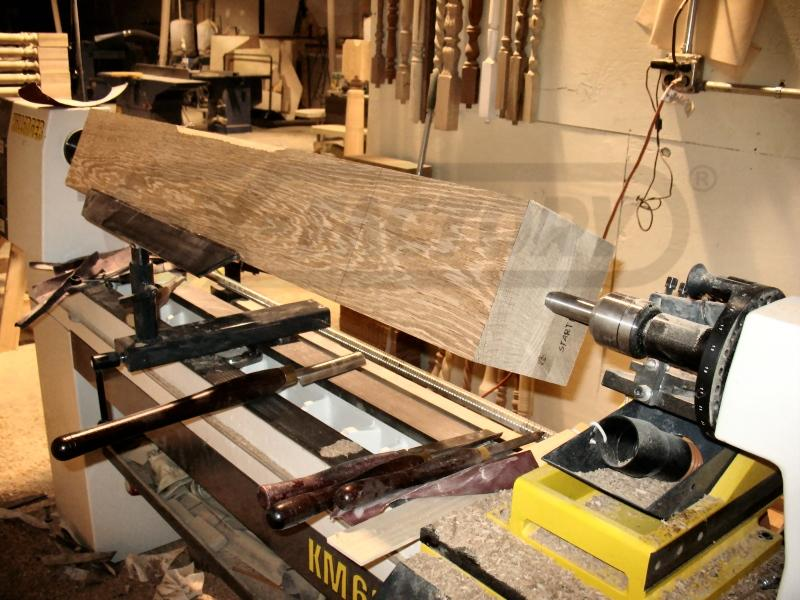
\includegraphics[height=2.5cm]{png/tour_bois}

\textit{Tour à bois \cite{tab}}
\end{center}
\end{minipage} \hfill
\begin{minipage}[c]{.23\linewidth}
\begin{center}
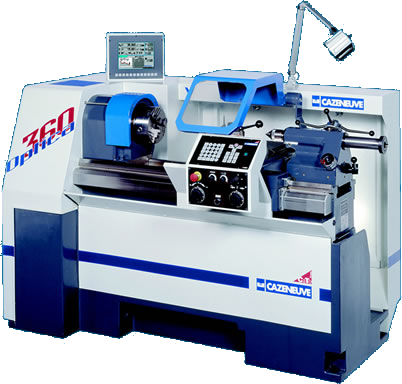
\includegraphics[height=2.5cm]{png/cazeneuve}

\textit{Tour conventionnel \cite{cazeneuve}}
\end{center}
\end{minipage} \hfill
\begin{minipage}[c]{.23\linewidth}
\begin{center}
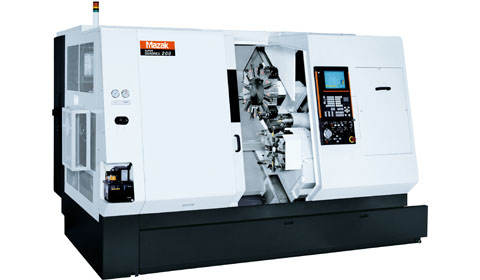
\includegraphics[height=2.5cm]{png/tour_mazak}

\textit{Tour à commande numérique \cite{mazak}}
\end{center}
\end{minipage}\hfill
\begin{minipage}[c]{.23\linewidth}
\begin{center}
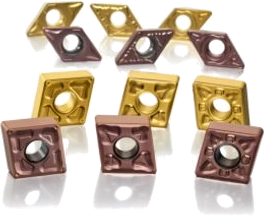
\includegraphics[height=2.5cm]{png/plaquettes}

\textit{Plaquettes de tournage \cite{plaquettes}}
\end{center}
\end{minipage}

\vspace{.5cm}

\begin{center}
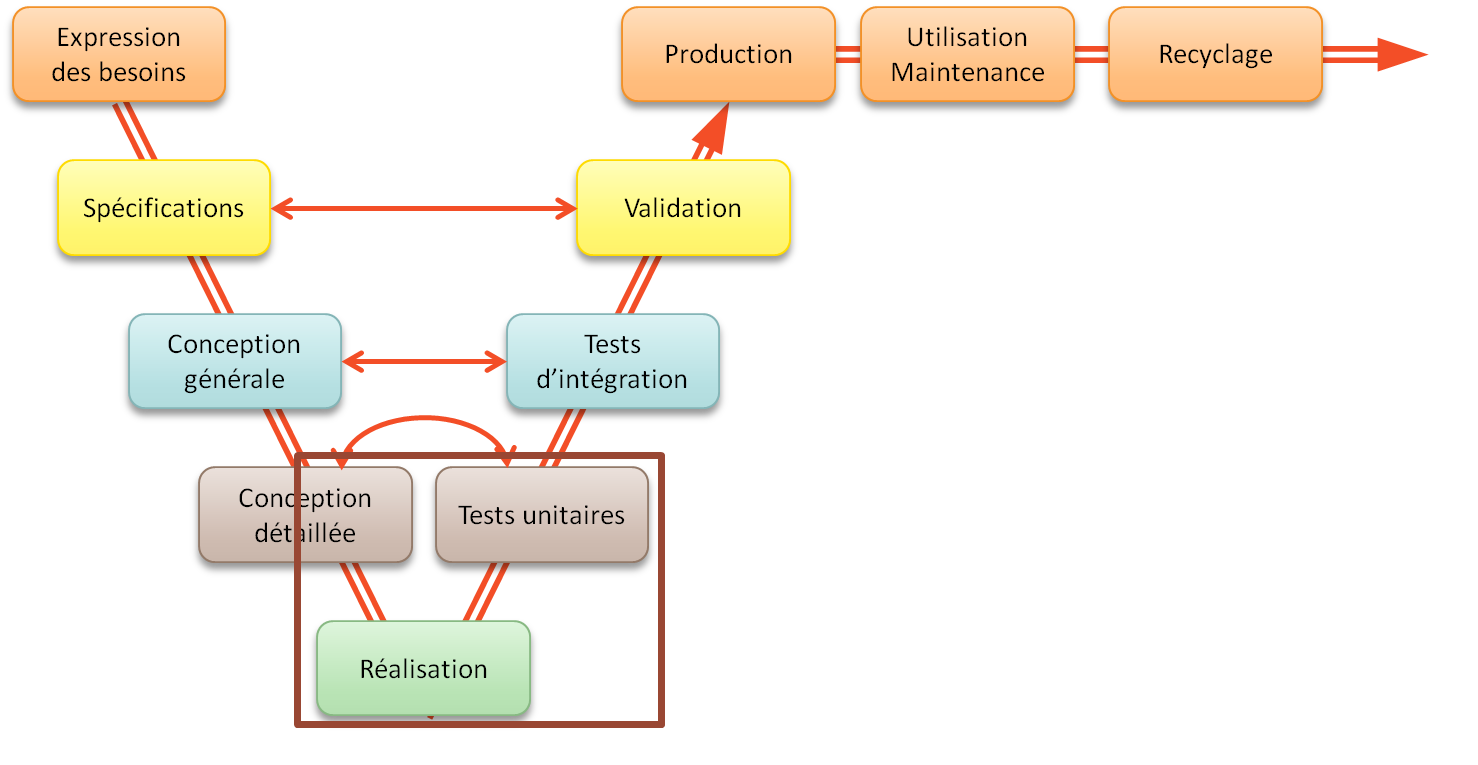
\includegraphics[height=7cm]{png/cycleV}
\end{center}

%\begin{center}
%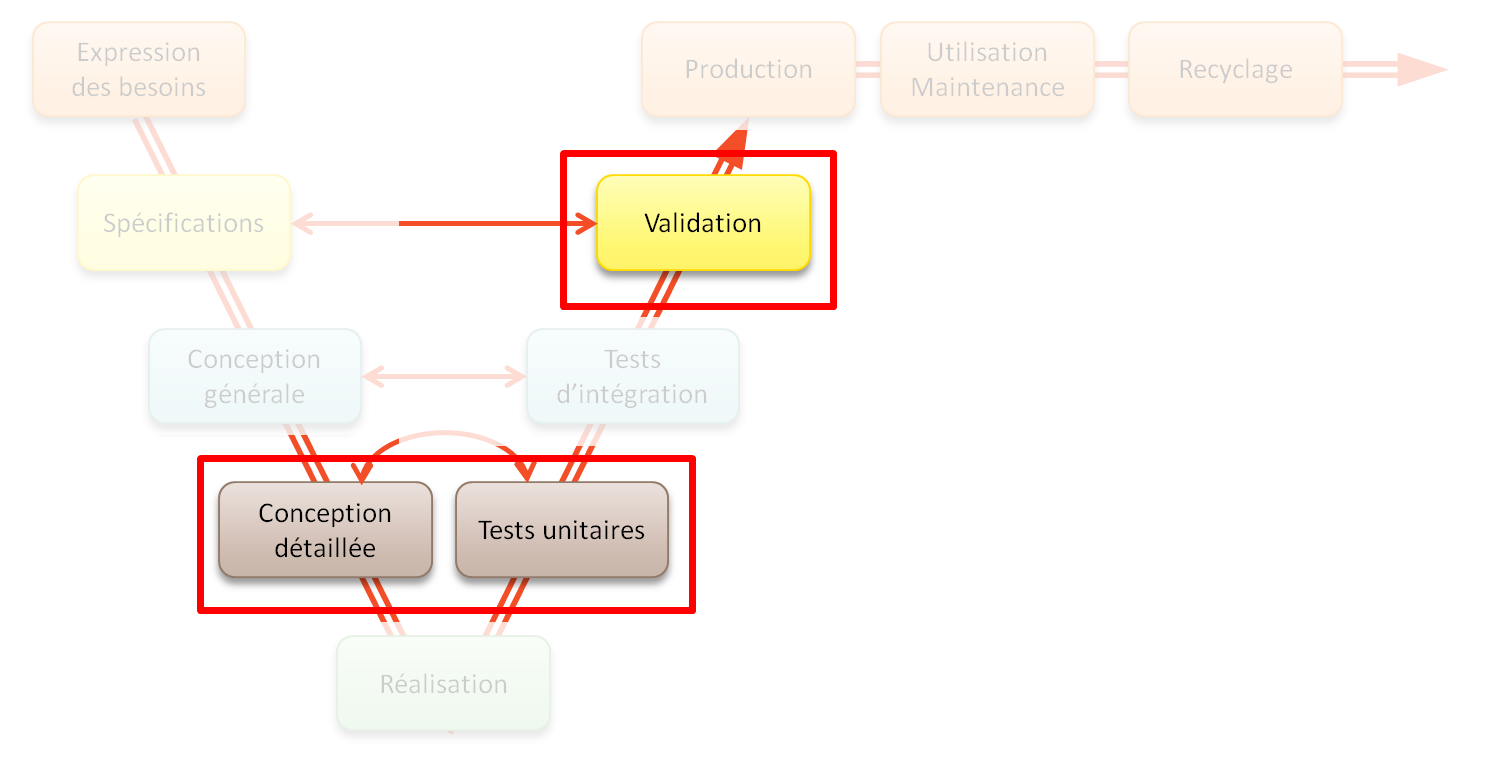
\includegraphics[width=.9\textwidth]{png/cyclev.png}

%\textit{Cycle de conception d'un produit}
%\end{center}

%\begin{prob}
%\textsc{Problématique :}
%\begin{itemize}
%\item %Quelles sont les conditions fonctionnelles permettant le fonctionnement du système ?
%\item %Quelle est la chaîne de côte unidirectionnelle correspondant à une condition donnée ?
%\end{itemize}
%\end{prob}



\begin{savoir}
\textsc{Savoirs :}
\begin{itemize}
\item Présenter de façon structurée un usinage en tournage :
\begin{itemize}
\item Les éléments de la cellule élémentaire d'usinage
\item Les opérations de tournage
\end{itemize}
\end{itemize}
\end{savoir}
 

\setlength{\parskip}{0ex plus 0.2ex minus 0ex}
 \renewcommand{\contentsname}{}
 \renewcommand{\baselinestretch}{1}

\tableofcontents

 \renewcommand{\baselinestretch}{1.2}
\setlength{\parskip}{2ex plus 0.5ex minus 0.2ex}

% \vspace{1cm}
\textit{Ce document évolue. Merci de signaler toutes erreurs ou coquilles.}

\section{Présentation}

\subsection{Définition}

\begin{defi}
\textbf{Tournage}

\begin{minipage}[c]{.55\linewidth}
Le tournage est une opération d'usinage qui permet de réaliser des surfaces de révolution. Le \textbf{mouvement de coupe} est assuré par une rotation de la pièce autour de l'axe de révolution. Le \textbf{mouvement d'avance} est assuré par des translations de l'outil dans un plan contenant l'axe de révolution. 
\end{minipage}\hfill
\begin{minipage}[c]{.4\linewidth}
\begin{center}
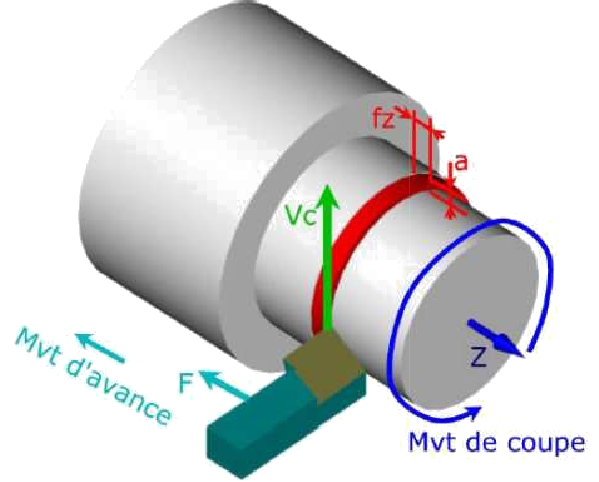
\includegraphics[width=.95\textwidth]{png/mvt_tournage}
\end{center}
\end{minipage}
\end{defi}


\subsection{Cellule élémentaire d'usinage}

\begin{minipage}[c]{.55\linewidth}
Les systèmes de production sont constitués des éléments suivants : 
\begin{itemize}
\item la machine : dans notre cas la machine est un tour. Il est dit conventionnel quand les déplacements des axes sont directement générés par un opérateur. Il est dit à commande numérique lorsque les déplacements des axes et la gestion de la machine se fait par une commande numérique, autrement dit, un ordinateur;
\item le porte-outil permet de faire l'interface entre la tourelle de la machine et l'outil; 
\item l'outil coupant permet de réaliser des opérations de tournage sur une pièce;
\item le porte pièce permet de faire l'interface entre la machine et la pièce;
\item la pièce est le produit à usiner. 
\end{itemize}
\end{minipage}\hfill
\begin{minipage}[c]{.4\linewidth}
\begin{center}
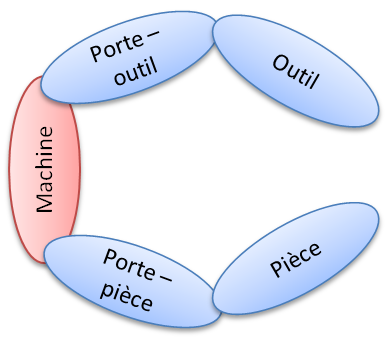
\includegraphics[width=.95\textwidth]{png/ceu}
\end{center}
\end{minipage}
\section{Les machines}
\subsection{Axes normalisés}
Sur les centres d'usinage, le choix des axes de déplacement est normalisé. Cela est notamment nécessaire dans le cas de la programmation des commandes numériques afin qu'un programme soit plus facilement transmissible d'une machine à une autre. 

Le nombre d'axes est donné par les mouvements d'avance. Le plus communément les tours sont des machines à \textbf{2 axes}.

D'après la norme :
\begin{itemize}
\item l'axe $\vect{Z_m}$ est parallèle à l'axe de rotation de la broche. Le sens positif est donné par l'éloignement de l'outil par rapport à la pièce;
\item l'axe $\vect{X_m}$ est perpendiculaire à l'axe $\vect{Z_m}$. Il a la direction du plus grand déplacement. Le sens positif est donné par l'éloignement de l'outil par rapport à la pièce;
\item l'axe $\vect{Y_m}$ est tel que le trièdre $(\vect{X_m},\vect{Y_m},\vect{Z_m})$ soit orthonormé direct. 
\end{itemize}

\begin{minipage}[c]{.45\linewidth}
\begin{center}
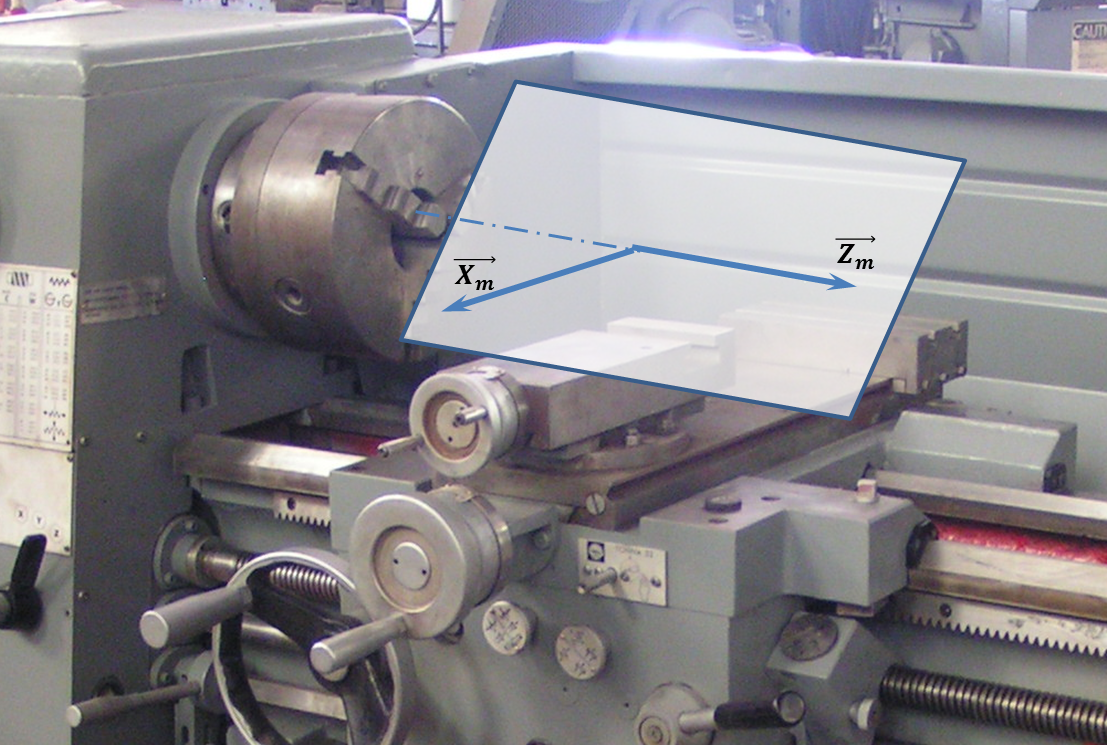
\includegraphics[height=4cm]{png/axes_normalises}

\textit{Axes normalisés sur un tour conventionnel}
\end{center}
\end{minipage}\hfill
\begin{minipage}[c]{.45\linewidth}
\begin{center}
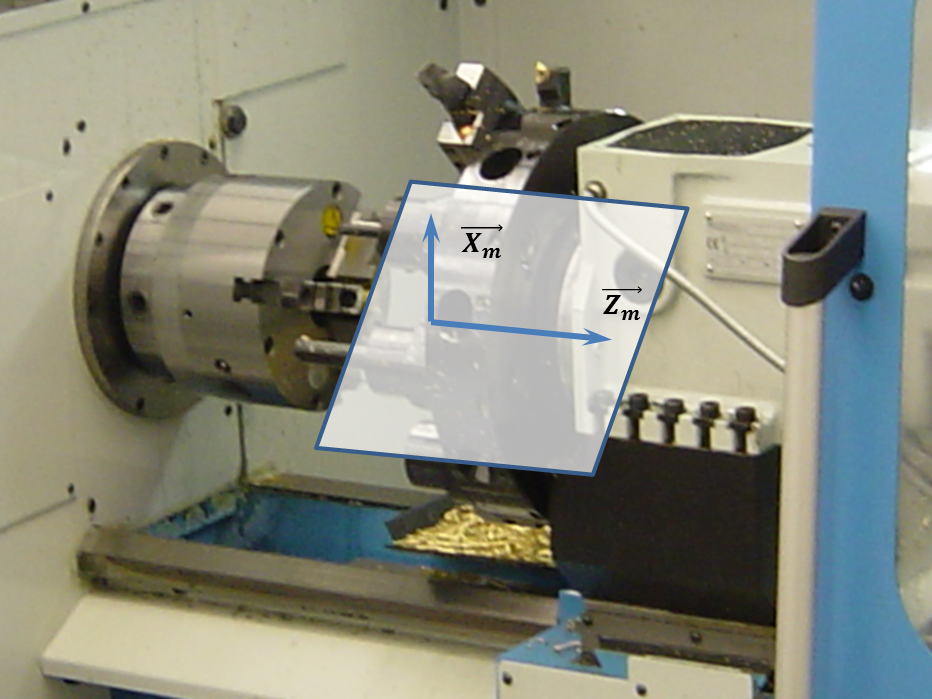
\includegraphics[height=4cm]{png/axes_normalises_2}

\textit{Axes normalisés sur un tour à commandes numériques}
\end{center}
\end{minipage}

On rencontre aussi couramment des tours à commande numérique 3 axes. Dans ce cas, le troisième axe est noté $\vect{C_m}$. Il s'agit d'un axe de rotation autour de l'axe $\vect{Z_m}$. Dans cette configuration, il est souvent possible de mettre un outil tournant dans le porte-outil puis d'indexer la position de la broche. Il est ainsi possible de réaliser un méplat sur un tour. 

Enfin, il existe des centres de tournage multi axes avec 3 axes de translations, des tourelles multiples ...

\subsection{Les machines conventionnelles}
Sur les machines conventionnelles, une fois la vitesse d'avance fixée, les distances de déplacement sont directement gérées par l'opérateur. 

Les mouvements des machines conventionnelles sont assurés par un moteur asynchrone. Elles sont équipées de deux  boîtes de vitesses mécaniques. La première permet de fixer la vitesse d'avance de l'outil. La seconde permet de choisir la fréquence de rotation de la broche. 

\begin{center}
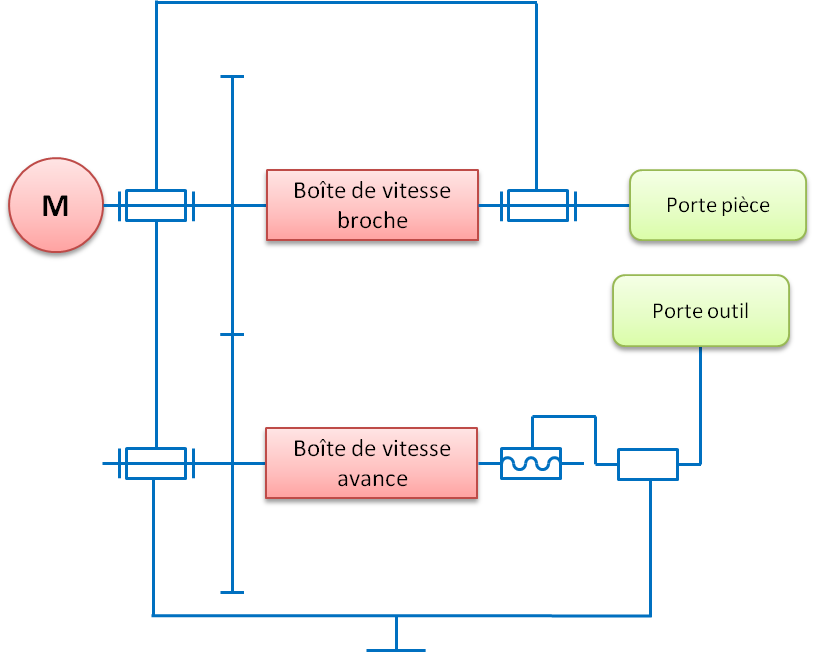
\includegraphics[width=.7\textwidth]{png/schema_tour_conv}
\end{center}


\subsection{Les machines à commandes numériques}
Les machines à commandes numériques sont équipées d'un moteur asynchrone pour la broche ainsi que d'un variateur de vitesse permettant un choix de vitesse plus précis qu'avec une boîte de vitesse. Deux autres moteurs à courants continus permettent de déplacer l'outil généralement sur deux axes ($\vect{X_m}$ et $\vect{Z_m}$). 

Par le fait, les mouvements des différents axes sont gérés par une commande numérique (ordinateur industriel). Ces mouvements sont générés grâce à des logiciels de fabrication assistée par ordinateur (FAO). Un post-processeur permet de convertir les programmes du langage FAO vers le langage CN. 

\begin{center}
\textit{Chaîne numérique}

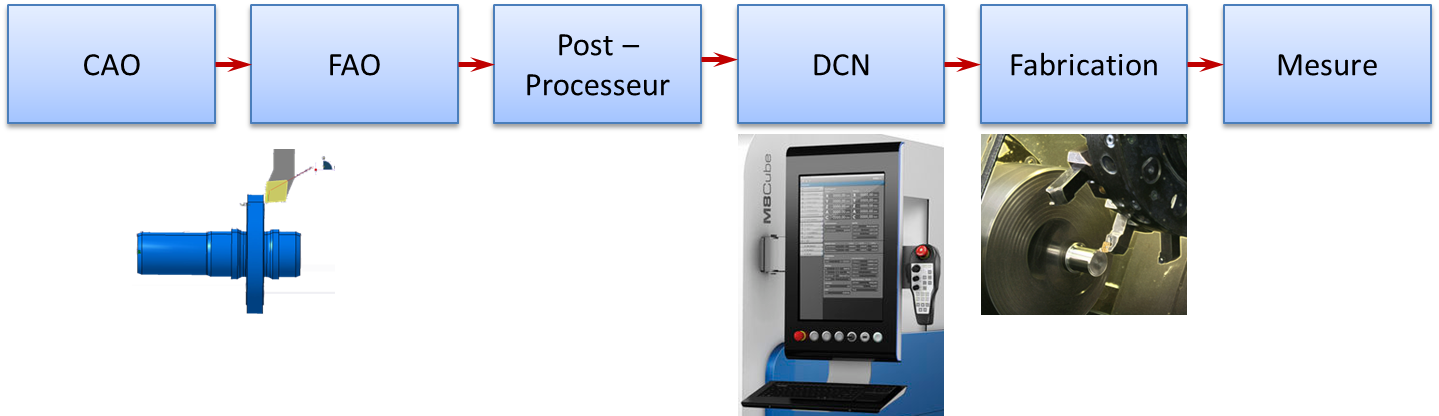
\includegraphics[width=.95\textwidth]{png/chaine_num}
\end{center}


\begin{center}
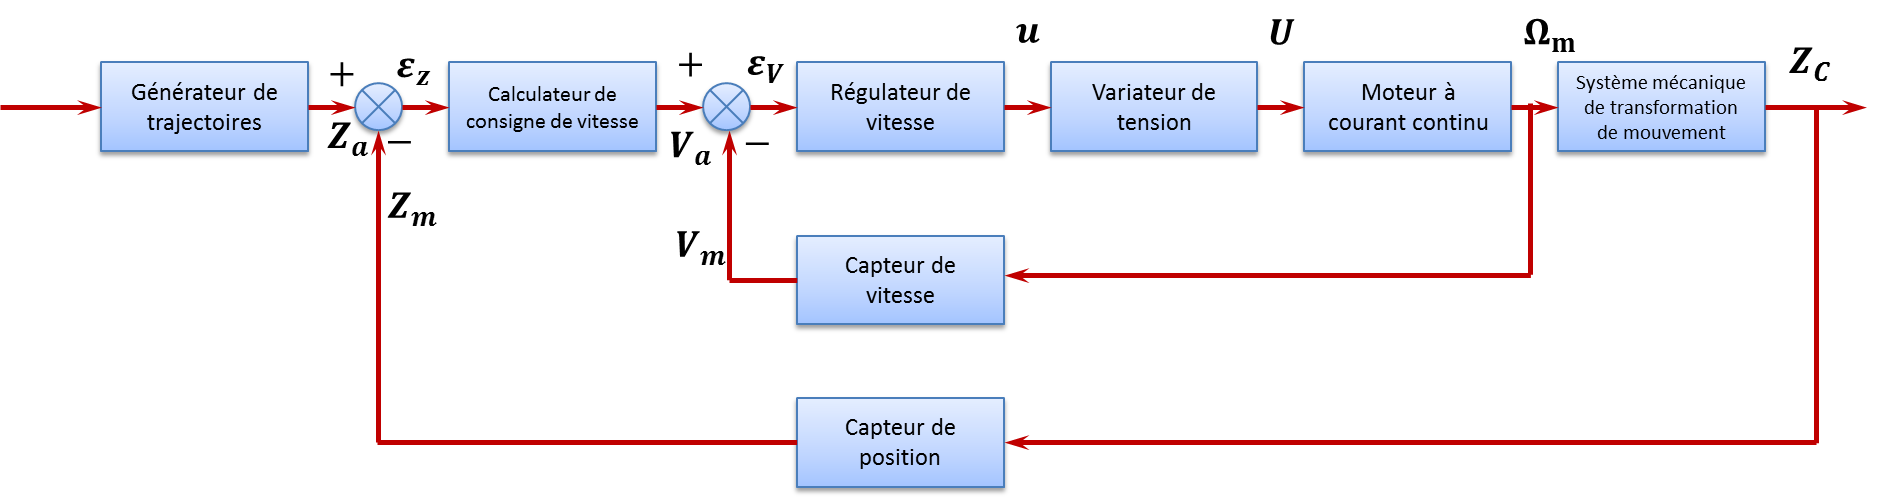
\includegraphics[width=.95\textwidth]{png/asservissement_cn}
\end{center}



\subsection{Les machines spéciales}
Industriellement, il existe des tours multibroches, multitrourelles avec embarreurs qui permettent d'avoir une très grande productivité. 



\begin{minipage}[c]{.3\linewidth}
\begin{center}
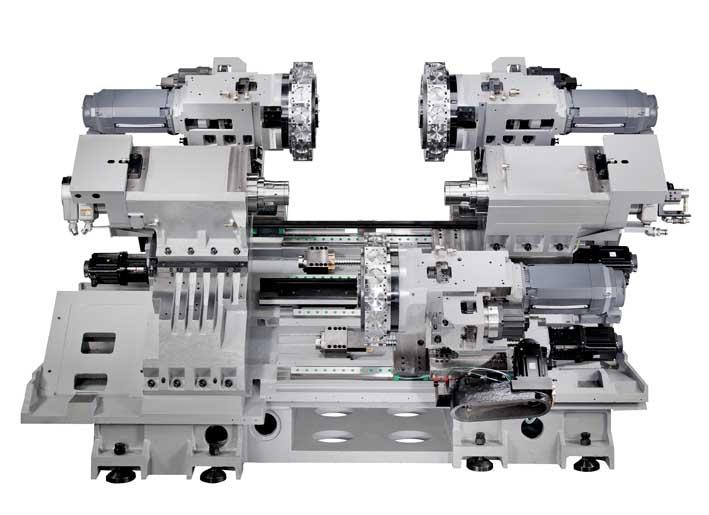
\includegraphics[height=4cm]{png/tour_multi_3}
\end{center}
\end{minipage}\hfill
\begin{minipage}[c]{.3\linewidth}
\begin{center}
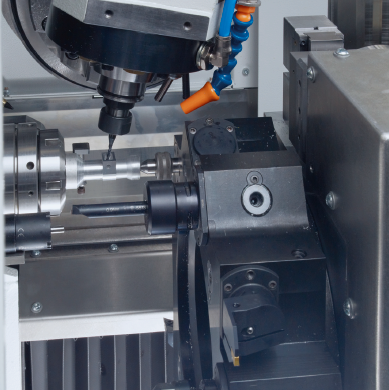
\includegraphics[height=4cm]{png/tour_multi_1}
\end{center}
\end{minipage}\hfill
\begin{minipage}[c]{.3\linewidth}
\begin{center}
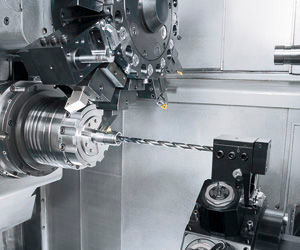
\includegraphics[height=4cm]{png/tour_multi_2}
\end{center}
\end{minipage}

\section{Typologie de pièces}
\section{Les porte-outils}

Sur un tour conventionnel ou numérique, la liaison entre le porte-outil et la machine s'appelle la tourelle. En usinage conventionnel, la tourelle ne peut contenir qu'un seul outil. La tourelle est orientable. En usinage à commande numérique, la tourelle peut porter plusieurs outils. 

\begin{minipage}[c]{.45\linewidth}
\begin{center}
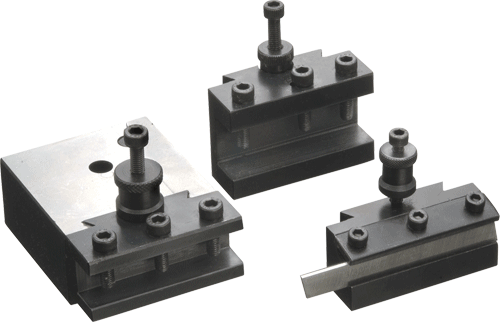
\includegraphics[height=4cm]{png/tourelle_2}

\textit{Tourelle de tour conventionnel}
\end{center}
\end{minipage}\hfill
\begin{minipage}[c]{.45\linewidth}
\begin{center}
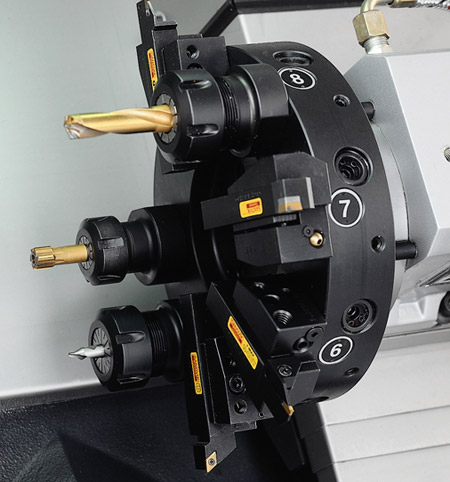
\includegraphics[height=6cm]{png/tourelle}

\textit{Tourelle de tour à commande numérique}
\end{center}
\end{minipage}


En usinage conventionnel, les outils à charioter-dresser sont maintenus en position par des vis sur le porte-outil. Le porte-outil est souvent mis en position grâce à un assemblage par queue d'aronde. Pour les outils à percer, on utilise un mandrin mis en position par adhérence (avec un cône morse) dans la contre pointe du tour. 

\begin{minipage}[c]{.45\linewidth}
\begin{center}
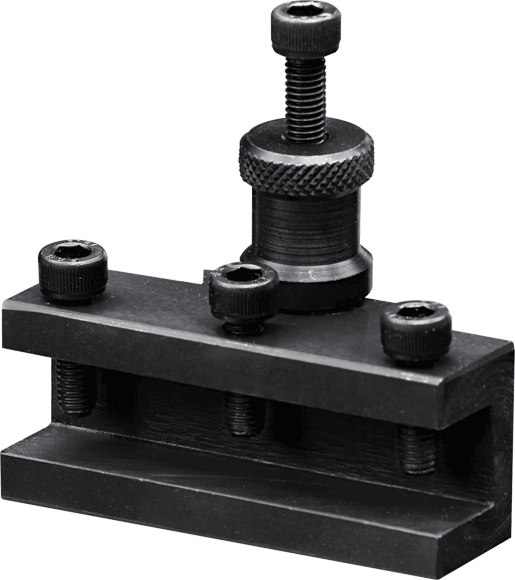
\includegraphics[height=3.5cm]{png/po_2}

\textit{Porte-outil carrés}
\end{center}
\end{minipage}\hfill
\begin{minipage}[c]{.45\linewidth}
\begin{center}
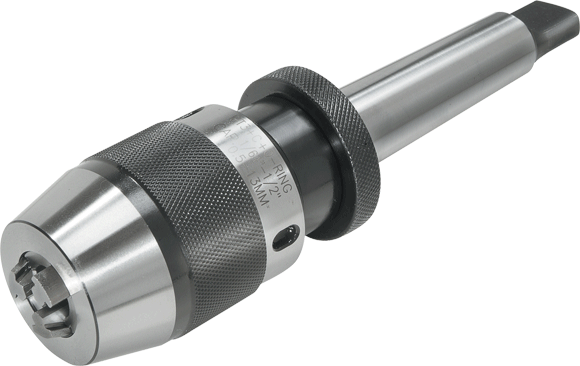
\includegraphics[height=3cm]{png/po_1}

\textit{Mandrins avec cône morse}
\end{center}
\end{minipage}


En usinage à commande numérique, le système d'attachement VDI est très utilisé. Pour les forets à centrer, à percer ou à aléser, on utilise en supplément des pinces qui permettent de serrer des outils ayant une base cylindrique. 


\begin{minipage}[c]{.3\linewidth}
\begin{center}
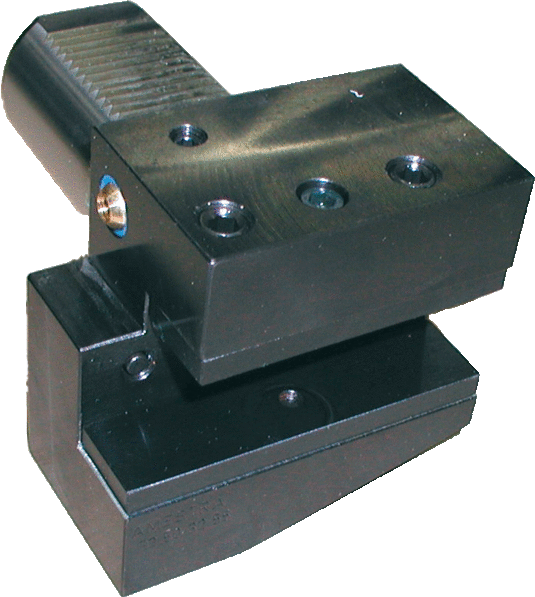
\includegraphics[height=3.5cm]{png/vdi_1}

\textit{Porte-outil pour outils à charioter et dresser}
\end{center}
\end{minipage}\hfill
\begin{minipage}[c]{.3\linewidth}
\begin{center}
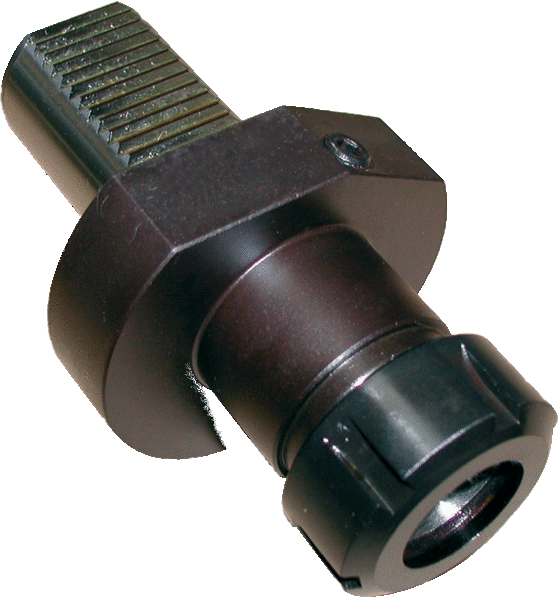
\includegraphics[height=3.5cm]{png/vdi_2}

\textit{Porte-outil pour outils à percer et aléser}
\end{center}
\end{minipage}\hfill
\begin{minipage}[c]{.3\linewidth}
\begin{center}
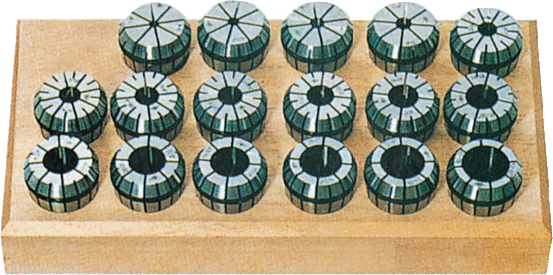
\includegraphics[height=2cm]{png/pinces}

\textit{Pinces pour outils à percer et aléser}
\end{center}
\end{minipage}

\section{Les outils}
\subsection{Géométrie des outils}

\begin{minipage}[c]{.65\linewidth}
En tournage, on utilise des outils monoblocs et des outils à plaquettes rapportées. Les outils monoblocs pour les opérations de type chariotage ou dressage, sont taillés spécifiquement en fonction des opérations à réaliser. Ils sont directement montés sur le porte outils carrés. 

Les outils permettant de réaliser les opérations de perçage possèdent une partie cylindrique qui leur permet de se monter dans des mandrins.
\end{minipage}\hfill
\begin{minipage}[c]{.3\linewidth}
\begin{center}
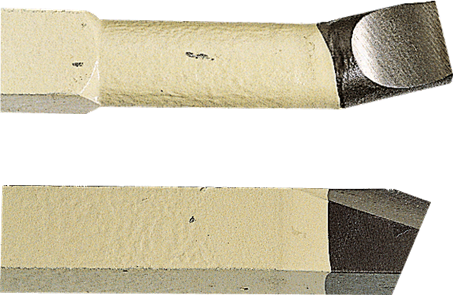
\includegraphics[width=.7\textwidth]{png/outils_hss}

\vspace{.5cm}

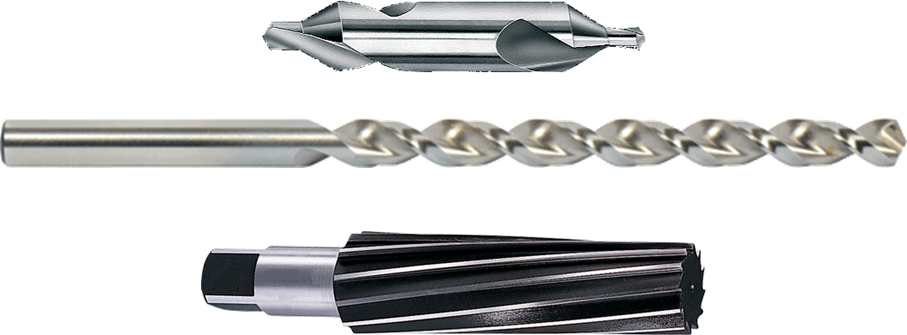
\includegraphics[width=\textwidth]{png/outils_hss_2}
\end{center}
\end{minipage}



\begin{minipage}[c]{.65\linewidth}
Pour les opérations de chariotage-dressage, lors de l'usinage en série, on utilise de préférence des plaquettes. Ces plaquettes peuvent être de formes variées : rondes, rhombiques, carrées ... avec des angles variés. Afin de faire la liaison avec les attachements on utilise des portes plaquettes. Pour une opération d'usinage, il faudra choisir une combinaison plaquette - porte plaquette dédiée. 
\end{minipage} \hfill
\begin{minipage}[c]{.3\linewidth}
\begin{center}
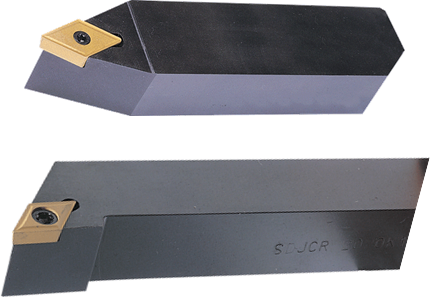
\includegraphics[width=.7\textwidth]{png/pp.png}

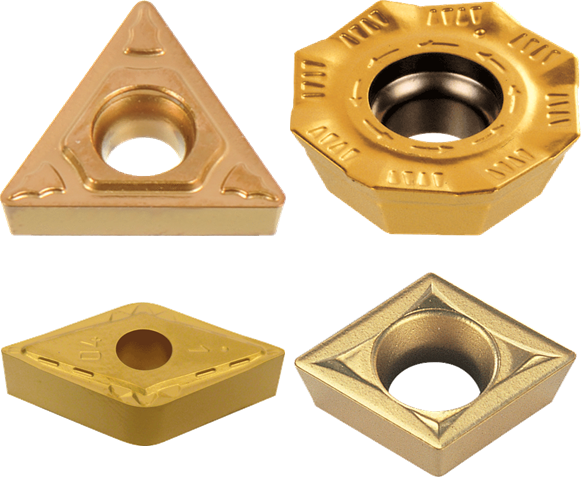
\includegraphics[width=.55\textwidth]{png/outils_plaq}
\end{center}
\end{minipage}




Pour une même plaquette, la géométrie du porte-plaquette peut permettre des usinages différents. Cependant, un mauvais choix de porte-plaquette peut provoquer des collisions entre la pièce et l'outil.

\begin{minipage}[c]{.45\linewidth}
\begin{center}
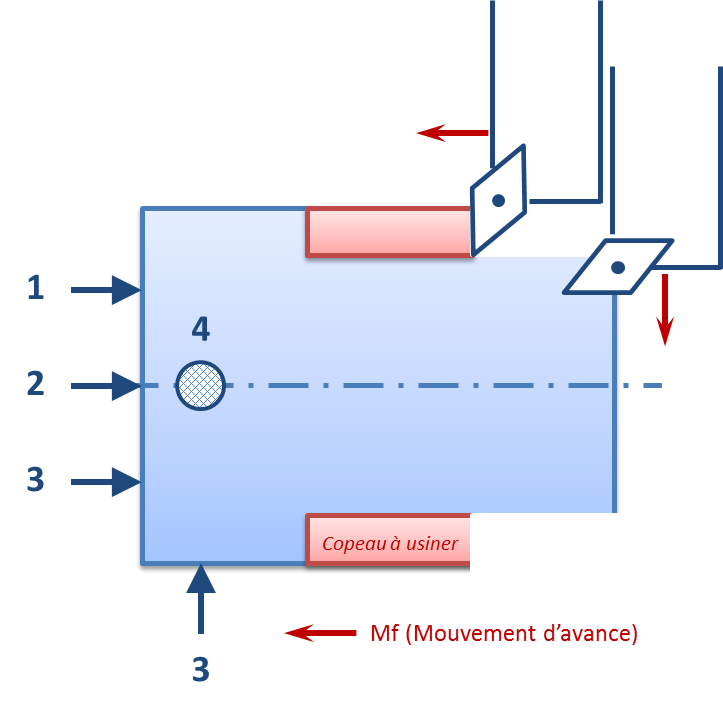
\includegraphics[width=.9\textwidth]{png/pp_geometrie.png}
\end{center}
\end{minipage} \hfill
\begin{minipage}[c]{.45\linewidth}
\begin{center}
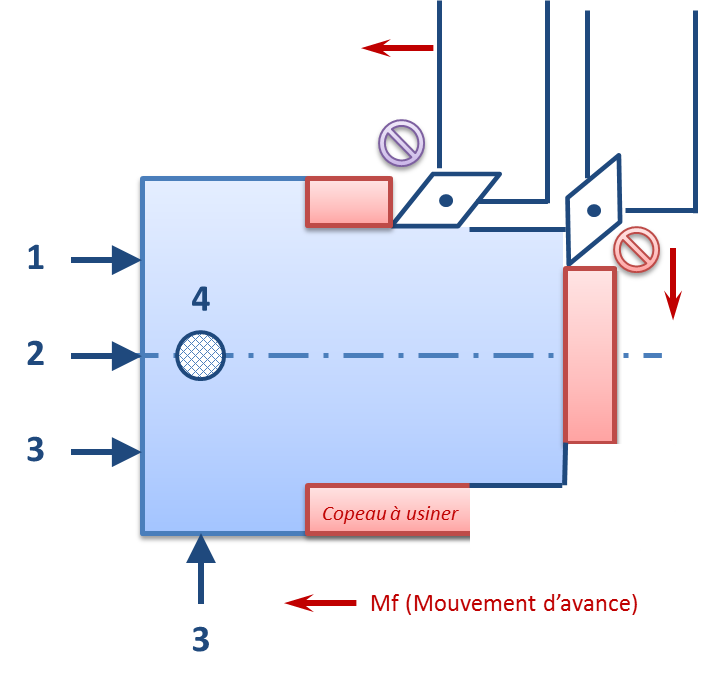
\includegraphics[width=.9\textwidth]{png/pp_geometrie_2.png}
\end{center}
\end{minipage} 


\subsection{Les opérations d'usinage}
\begin{center}
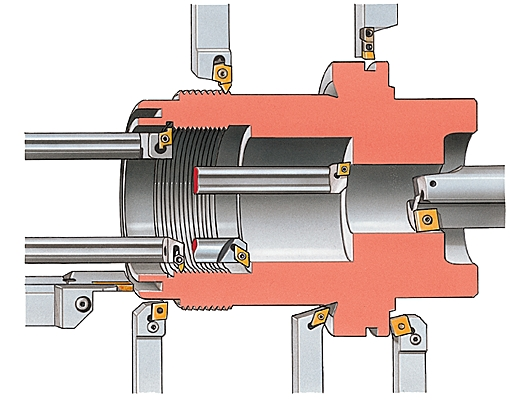
\includegraphics[width=.55\textwidth]{png/op_tournage}
\end{center}
\subsubsection{Dressage}
\begin{center}
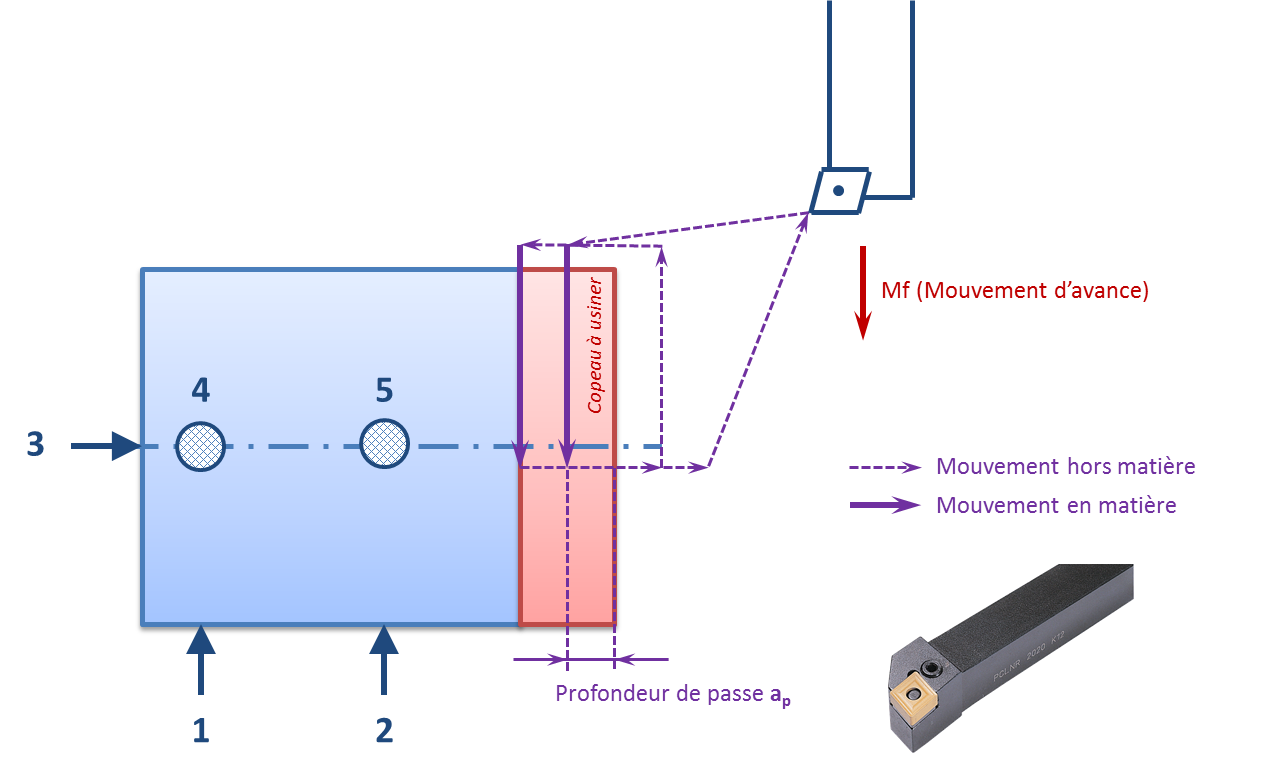
\includegraphics[width=.7\textwidth]{png/op_dressage}
\end{center}
\subsubsection{Chariotage}
\begin{center}
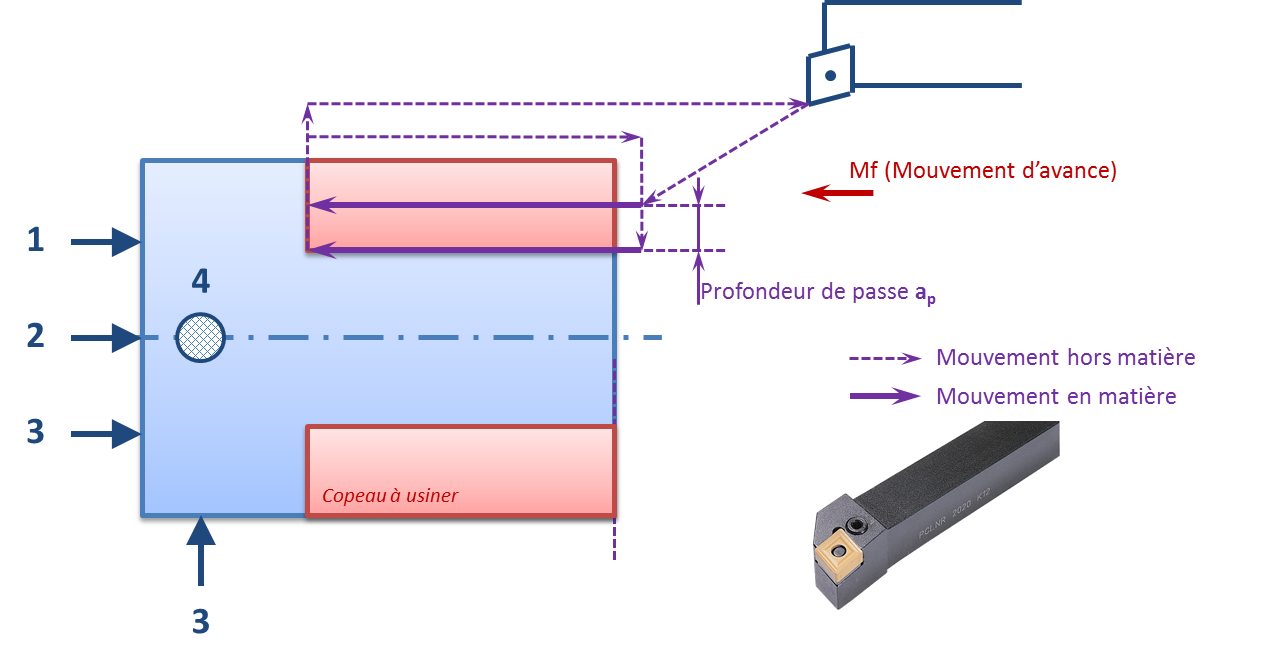
\includegraphics[width=.7\textwidth]{png/op_chariotage}
\end{center}
\subsubsection{Chanfreinage}
\begin{center}
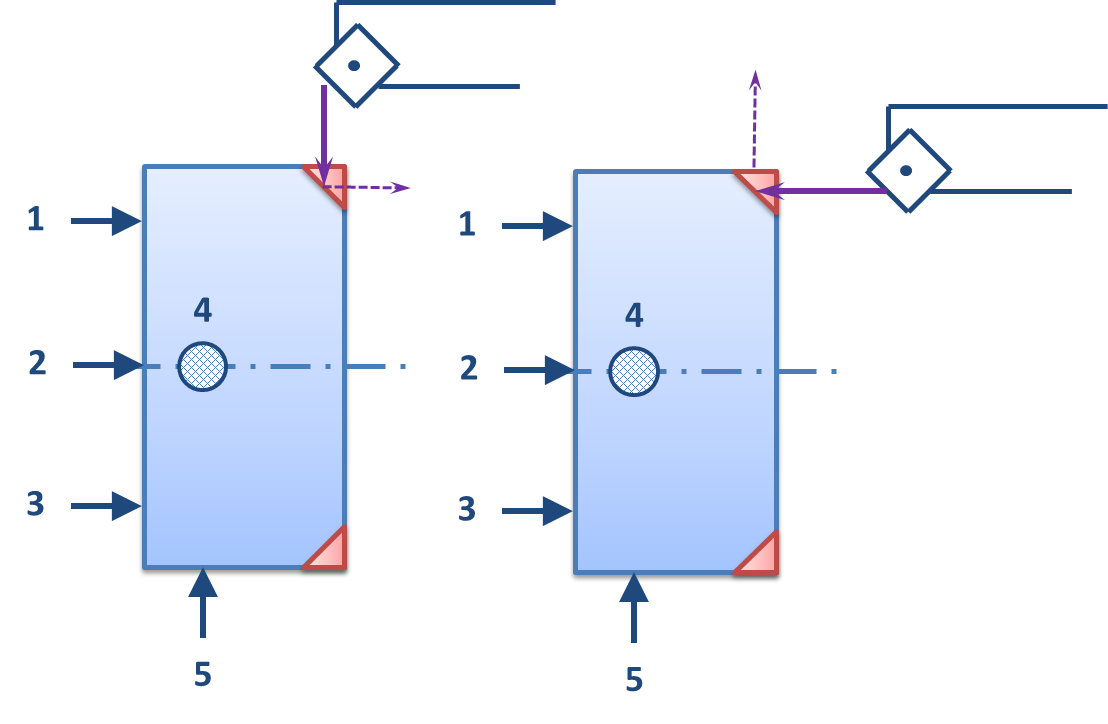
\includegraphics[width=.7\textwidth]{png/op_chanfrein}
\end{center}
\subsubsection{Perçage}
\begin{center}
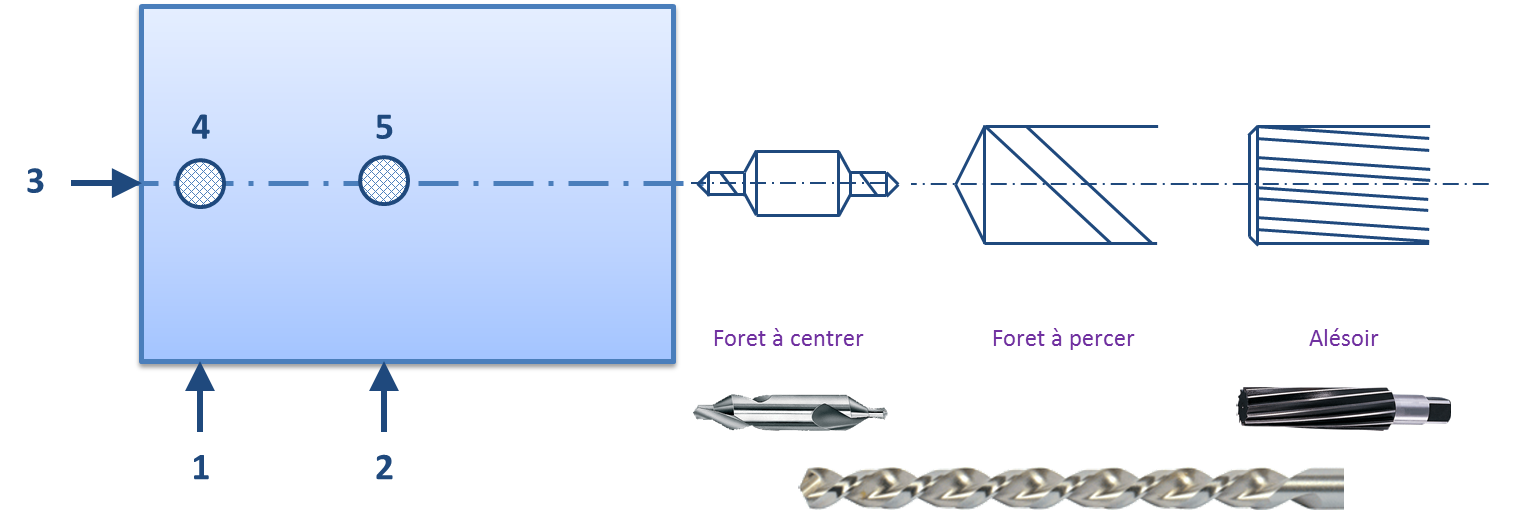
\includegraphics[width=.7\textwidth]{png/op_percage}
\end{center}
\subsubsection{Tronçonnage et gorges}
\begin{center}
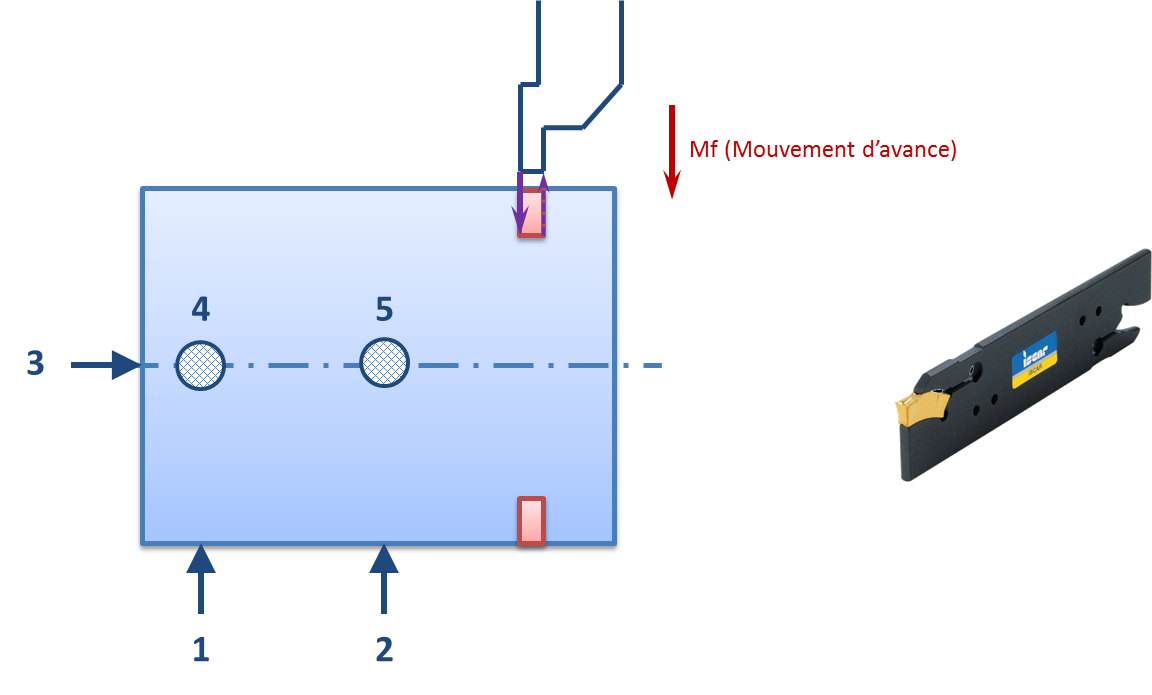
\includegraphics[width=.7\textwidth]{png/op_gorge}
\end{center}
\subsubsection{Filetage}
\begin{center}
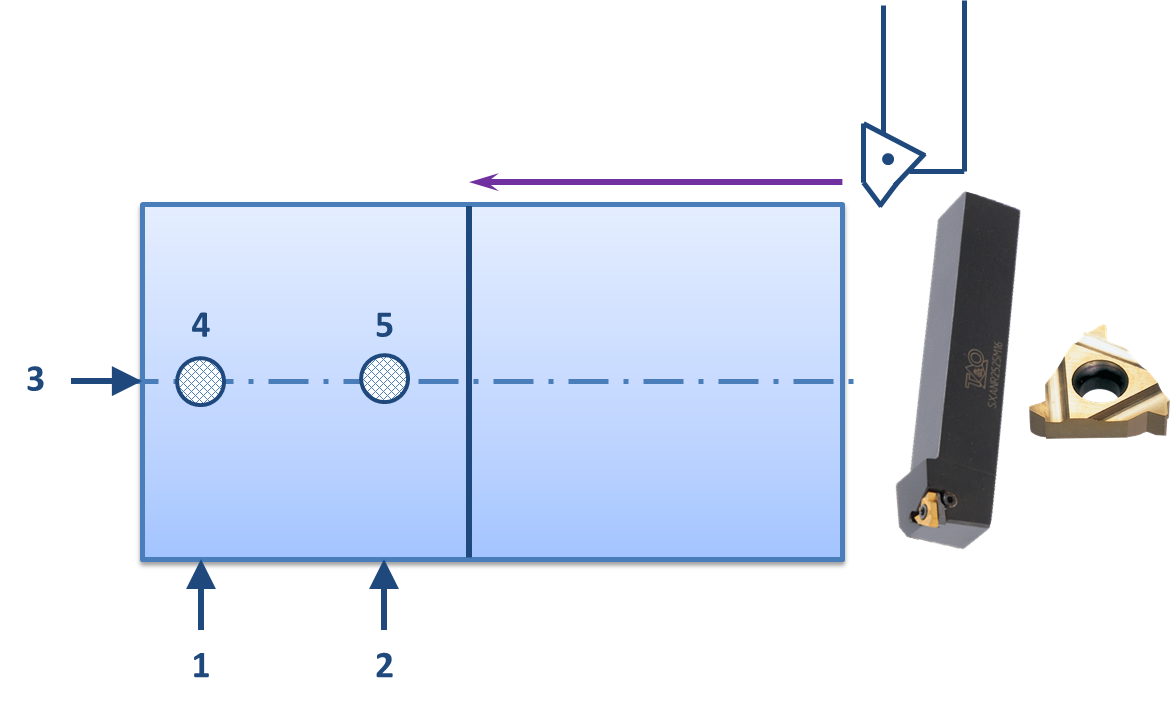
\includegraphics[width=.7\textwidth]{png/op_filetage}
\end{center}

\begin{center}
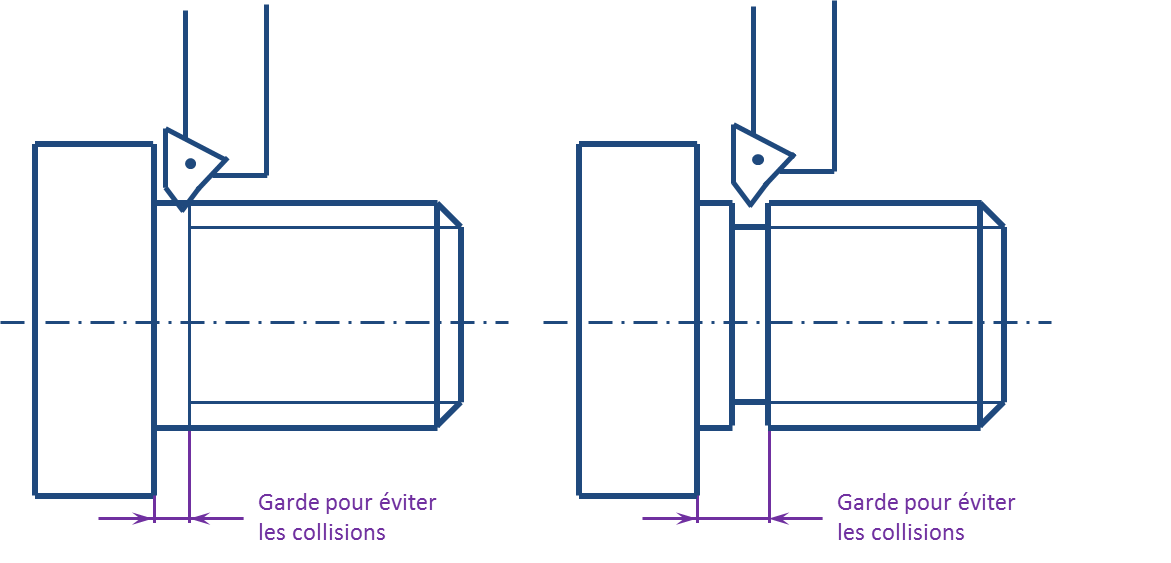
\includegraphics[width=.7\textwidth]{png/op_filetage2}
\end{center}

%\subsubsection{Opérations particulières}
%Méplats...


\section{Les portes pièces}
\subsection{Cahier des charges}

\begin{center}
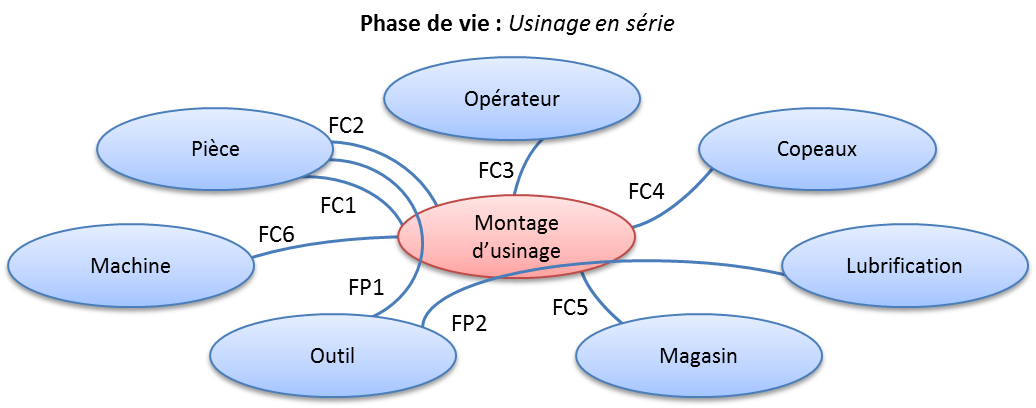
\includegraphics[width=.95\textwidth]{png/af1}
\end{center}

\begin{center}
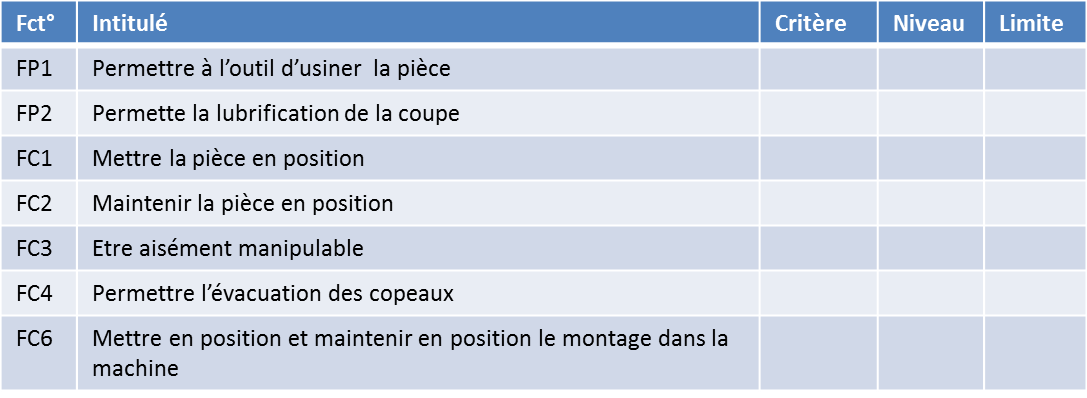
\includegraphics[width=.95\textwidth]{png/af2}
\end{center}


\subsection{Les portes pièces}
\begin{minipage}[c]{.45\linewidth}
\begin{center}
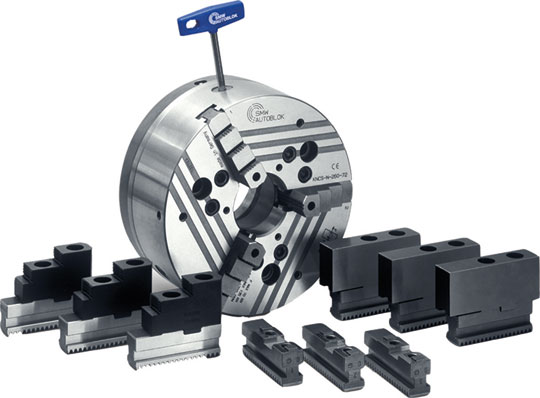
\includegraphics[width=.9\textwidth]{png/mandrin}

\textit{Mandrins et mors de serrages}
\end{center}
\end{minipage}\hfill
\begin{minipage}[c]{.45\linewidth}
\begin{center}
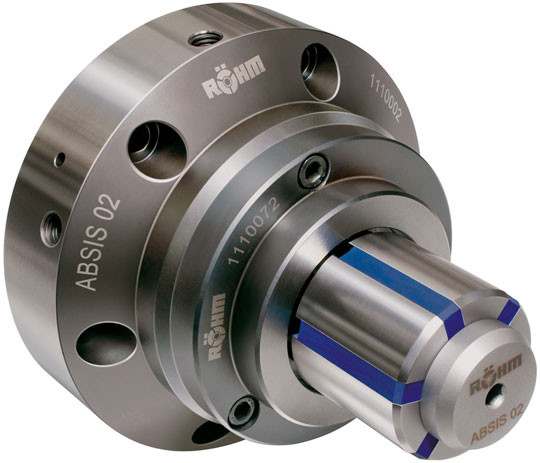
\includegraphics[width=.6\textwidth]{png/mandrin_exp}

\textit{Mandrin expansible}
\end{center}
\end{minipage}

\subsection{Mise en position isostatique des pièces}
Sur un contrat de phase (voir partie suivante), il est nécessaire d'indiquer comment sera positionnée la pièce dans la machine. Cette mise en position est indépendante du porte-pièce. Il ne s'agit que d'une représentation symbolique.

La mise en position de la pièce permet de mettre en évidence comment sera réalisée la liaison encastrement entre la pièce et le porte-pièce. Afin de réaliser une liaison encastrement, il faut bloquer 6 degrés de liberté qui seront représentés par des flèches numérotées. 

\begin{warn}
Lors de montage  \textbf{en mandrin}, on ne cherchera à supprimer que 5 degrés de liberté. La rotation de la pièce autour de son axe sera bloquée par le serrage du mandrin. 
\end{warn}

Le choix de la mise en position dépend :
\begin{itemize}
\item de la cotation de la pièce;
\item de l'étendue des surfaces;
\item de l'accessibilité des surfaces.
\end{itemize}


En tournage, les mises en positions les plus courantes sont les suivantes : 

\begin{minipage}[c]{.48\linewidth}
\begin{center}
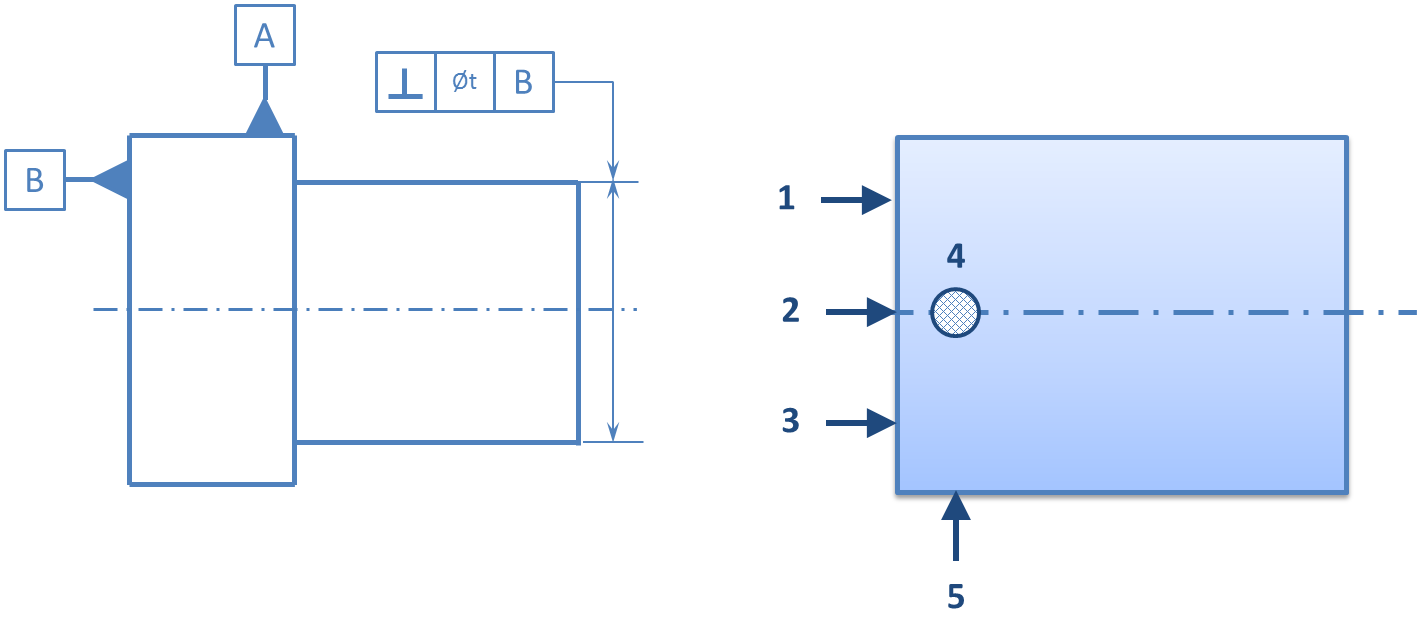
\includegraphics[width=\textwidth]{png/MIP_2}

\textit{MIP par appui plan et centrage court}
\end{center}
\end{minipage}\hfill
\begin{minipage}[c]{.48\linewidth}
\begin{center}
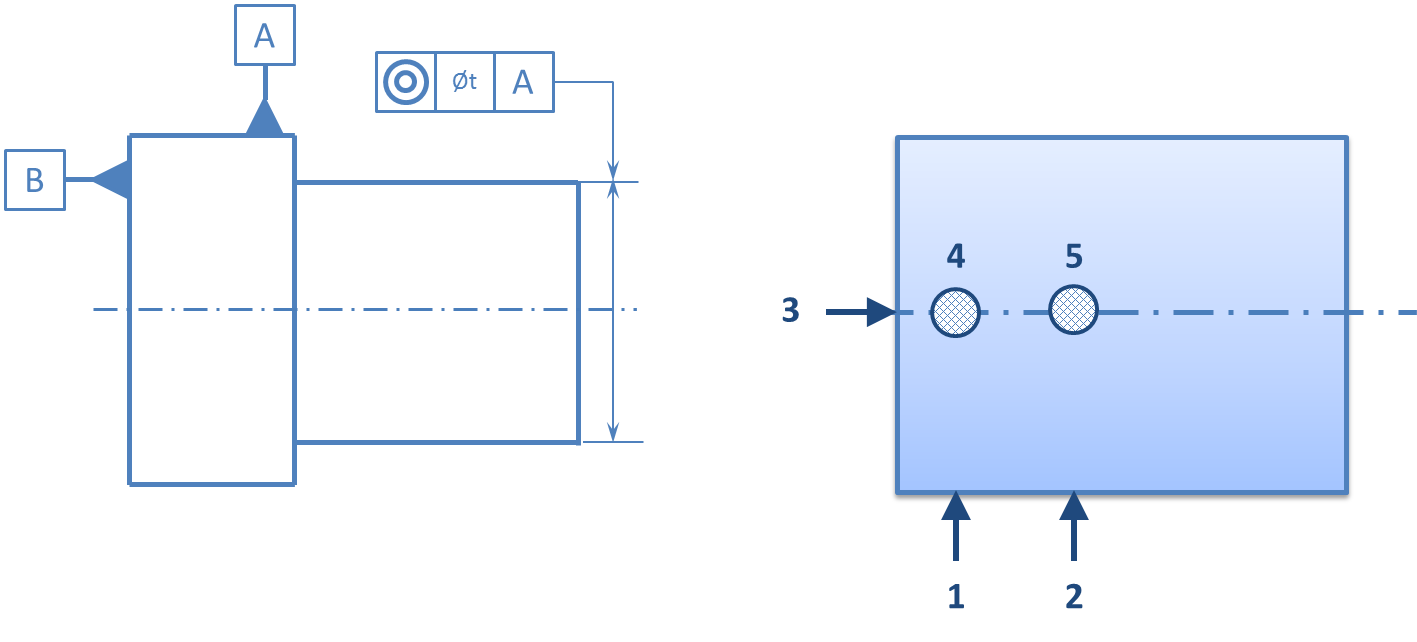
\includegraphics[width=\textwidth]{png/MIP_1}

\textit{MIP par cylindre prépondérant et appui ponctuel}
\end{center}
\end{minipage}

Technologiquement, chacun des appuis est généralement réalisé par les mors. Dans certain cas la face du mandrin peut servir d'appui plan. Dans certains cas, une pige à l'intérieur du mandrin permet de réaliser un appui ponctuel.




\begin{minipage}[c]{.4\linewidth}

Pour les pièces longues, il est possible de réaliser un montage entre pointes. Cela permet de diminuer le défaut de forme provoquer par la flexion de la pièces lors de l'usinage. On utilise alors la contre pointe située dans la poupée mobile. 

\end{minipage}\hfill
\begin{minipage}[c]{.48\linewidth}
\begin{center}
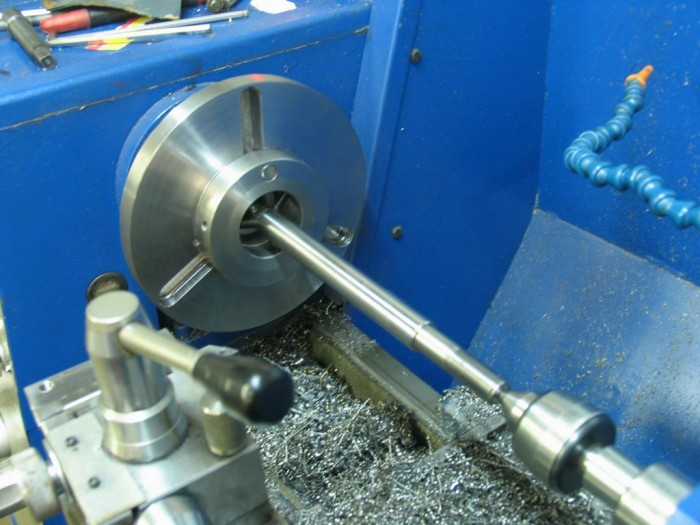
\includegraphics[width=.8\textwidth]{png/entre_pointes}
\end{center}
\end{minipage}

Enfin, il existe des montages spécifiques en tournage qui sont spécialement conçus et fabriqués pour certains types de pièces. 


\section{Contrat de phase}
\begin{defi}
Un contrat de phase est un document comportant toutes les opérations présentes dans une phase. Une phase correspond à un posage (une mise en position) unique de la pièce.
\end{defi}
\subsection{Ordonnancement des phases}

On désire réaliser la pièce suivante à partir d'un brut cylindrique :
\begin{center}
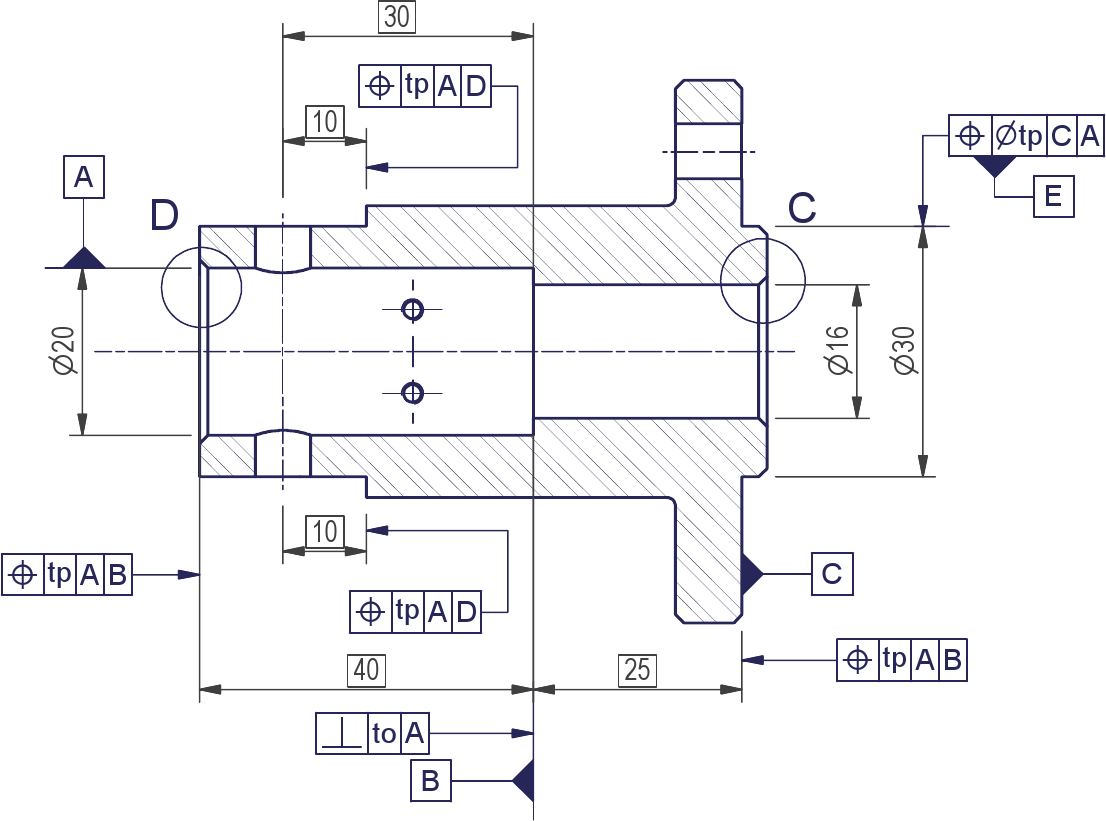
\includegraphics[width=.7\textwidth]{png/moyeu}

\textit{Dessin de définition partie du moyeu Speed'O'Kart}
\end{center}

Pour usiner la pièce, deux solutions semblent possibles initialement. Commencer par la partie "gauche" ou par la partie "droite". 
 
\begin{methode}
Pour choisir comment ordonnancer les phases, il est nécessaire de s'appuyer sur les spécifications.  Dans la mesure du possible on commence par usiner \textbf{les surfaces de références} des spécifications.

Les surfaces de références devront alors être utilisées pour réaliser la \textbf{mise en position de la pièce} lors de l'usinage des surfaces spécifiées.
\end{methode}


\subsection{Ordonnancement des opérations}
Il n'existe pas forcément de méthode rigoureuse pour ordonnancer les opérations. Le bon sens est souvent de rigueur. 

Lorsqu'il faut enlever une grande quantité de matière on commencera par réaliser une ébauche pour enlever une grande quantité de matière et avec le plus grand débit possible pour être productif. Une finition permettra alors d'obtenir la dimension finale et la qualité de surface souhaitée.

\subsection{Conditions de coupe}

\begin{defi}
\textbf{Conditions de coupe}

En tournage déterminer les conditions de coupe revient à déterminer : 
\begin{itemize}
\item la vitesse de coupe;
\item la vitesse d'avance; 
\item la profondeur de passe. 
\end{itemize}
\end{defi}

\begin{defi}
\textbf{Vitesse de coupe}

La vitesse de coupe correspond à la vitesse de l'arrête de coupe par rapport à la pièce. 

Elle est donnée par le couple outil matière, c'est-à-dire par la combinaison du matériau de l'outil et de la pièce. On la note $V_c$ et s'exprime en $m/min$. La vitesse de coupe permet de déterminer la vitesse de rotation de la broche. On la note $N$ en $tr/min$. 

On montre aisément que 
$$
N= \dfrac{1000\cdot V_c}{\pi D}
$$

Dans cette formule, $N$ est exprimé en $tr/min$, $V_c$ en $m/min$ et $D$ en $mm$.
\end{defi}

%% Vitesse de coupe

\begin{defi}
\textbf{Vitesse d'avance}

La vitesse d'avance correspond à la vitesse d'avance de l'outil sur la trajectoire d'usinage. On note $f$ la vitesse d'avance en $mm/tr$. Elle est choisie de manière à ce que le copeau fragmente correctement. En effet, un copeau court est préférable en tournage. Elle peut aussi être adaptée afin d'avoir l'état de surface souhaité en finition. 

La vitesse d'avance $V_f$ en $mm/min$ est donnée par $V_f = N\cdot f$.
\end{defi}

%% Détermination de la vitesse d'avance, diagramme brise copeau.

\begin{defi}
\textbf{Profondeur de passe}

Le choix de la profondeur de passe dépend de plusieurs paramètres. On la note $a$ en $mm$. Généralement, elle ne dépasse pas le tiers de la longueur de l'outil. 
Un choix judicieux de la profondeur de passe peut permettre d'augmenter la productivité. 

Cependant une grande profondeur de passe demande de plus grand efforts de coupe. Il faut alors que les efforts générés soient compatibles avec la puissance de la machine.
	
\end{defi}

\newpage 

\begin{thebibliography}{2}
\bibitem{tab}{\url{http://bois.fordaq.com/fordaq/srvAuctionView.html?AucTIid=17877844}}
\bibitem{cazeneuve}{\url{http://www.cazeneuve.fr/Cazeneuvefr/produits/Photos/Grandes/Optica360g.jpg}}
\bibitem{mazak}{\url{http://www.mazak.eu/fr/node/1087}}
\bibitem{plaquettes}{\url{http://www.industrie-techno.com/plaquettes-de-tournage-a-large-spectre-d-utilisation.13121}}
%\bibitem{cf}{\textit{La cotation fonctionnelle}, PTSI -- Lycée Vauban, Brest.}
%\bibitem{gdi}{\textit{Guide du dessinateur industriel}, André Chevalier, Éditions Hachette Technique, Editions 2004.}
%\bibitem{jpp}{Supports de cours de Jean-Pierre Pupier, Lycée Rouvière, Toulon.}
%\bibitem{gps}{\textit{Centre d'Études et de Rénovation Pédagogique de l'Enseignement Technique}, Exploitation du concept G.P.S. et de la normalisation pour la Spécification Géométrique des Produits.}
%\bibitem{gps2}{\textit{Le Décodage du Dessin de Définition}, Guy Percebois, Lycée Louis Vincent -- Metz . \url{http://www.ac-nancy-metz.fr/enseign/sti/genimeca/zip/GPS/Tol\%20g\%E9o\%20pr\%E9\%20bac.pdf}}
%\bibitem{rb}{Supports de cours de Renan Bonnard,PTSI, Lycée Newton, Clichy la Garenne}
%\bibitem{jb}{Supports de cours de Joël Boiron, PTSI, Lycée Gustave Eiffel, Bordeaux}
%\bibitem{mc}{Supports de cours de Maryline Carrez, Lycée Jules Haag, Besançon}
%\bibitem{pf}{Supports de cours de Philippe Fichou, Lycée Vauban, Brest \url{http://philippe.fichou.pagesperso-orange.fr/documents/liaisoncomplete2003.pdf}}
\bibitem{larousse}{\url{http://www.larousse.fr/encyclopedie/data/images/1001962-Tournage.jpg}}
\bibitem{mandrin}{\url{http://www.machine-outil.com/gfx/produits/grand/1601-mandrin-tour-smw-autoblok.jpg}}
\bibitem{mandrin}{\url{http://www.machine-outil.com/gfx//photos/grand/4257-mandrin-expansible-rohm.jpg}}
\bibitem{mandrin_exp}{\url{http://www.realmeca.com/upload/c60ab_tourelle_8positions.jpg}}
\bibitem{otelo}{\url{http://www.otelo.fr}}
\end{thebibliography}

\end{document}